\documentclass[prl,onecolumn,amsmath,amssymb,titlepage,nofootinbib,preprint]{revtex4-1}
	\usepackage{graphicx}
	%\usepackage{pslatex}	% to use PostScript fonts
	\usepackage{dcolumn}	% Align table columns on decimal point
	\usepackage{bm}			% bold math
	\usepackage[USenglish]{babel}	%spelling.... I think
	\usepackage{braket} 	% for bra's and ket's in math mode
 	\usepackage{multirow}	% for \tableofcontents
	\usepackage{setspace}	%NOTE: I don't know what this one is for.....
	\usepackage{fancyhdr}	%dat fancy header
	\usepackage{hyperref}	%hyperlink references
	\usepackage{sidecap}	%captions on the side
	\usepackage{mathrsfs}	%fancy fonts, not really needed
	\usepackage{subcaption} %used to create subfigure figures
	\usepackage{verbatim}   %block comments
	\pagestyle{fancy}
	
	

\begin{document}

%**************************************************************************************
	\title{Observation of Efimov's Scenario in Ultracold Atomic Gases}
	\author{Stephen J. Hageman}
	\email{hageman.65@osu.edu}
	\affiliation{Department of Physics, The Ohio State University, Columbus, OH 43210}
	\date{August 4, 2014}

	\begin{comment}
	\begin{abstract}
		Here is my abstract abstract.
	\end{abstract}
	\end{comment}

	\begin{figure}[b]
		
\includegraphics[width=0.05\textwidth]{Figures/BlockO}
	\end{figure}

	\maketitle
	\thispagestyle{empty}

%**************************************************************************************

\section{Introduction}
	\setcounter{page}{1}	%set page number so 1 is second
	Historically, the problem of three interacting bodies has been as intriguing as it has been difficult to solve.  The  study of such problems has attracted the likes of Leonhard Euler, Joseph-Louis Lagrange, Henri Poincar\'{e}, and many others.  In 1970, a Russian physicist at the Ioffe Institute in Leningrad was also drawn to the three-body problem in quantum mechanics.  Vitaly Efimov specialized in nuclear physics\footnote{He is currently an Affiliated Professor of nuclear theory at the University of Washington.}, and he was inspired by the work of L.H. Thomas on the triton (tritium nucleus) \cite{Thomas1935}.  Efimov's work culminated in a series of papers in the early seventies \cite{Efimov1970}\cite{Efimov1971}\cite{Efimov1979} which describe the peculiar behavior of a three-body system consisting of identical bosons.  His prediction was that in the presence of a resonant two-body interaction the three-body system would develop an infinite spectrum of bound trimers.  What made this result particularly surprising was that so long as the two-body interaction was sufficiently resonant the specific details of the inter-particle forces were not relevant.  Therefore, these Efimov states were predicted to be a universal property of the quantum mechanical three-body problem.
	
	Of course, the true test of any theory is experimental confirmation, and despite their claimed universality, empirical evidence for Efimov trimers remained elusive.  Efimov, as a nuclear physicist, originally proposed to search for their existence in nuclear systems such as tritons and halo nuclei \cite{Efimov1970}\cite{Efimov1971}. However, while there has been suggestive evidence, nothing truly conclusive has emerged from this approach \cite{Braaten_2006}.  The actual confirmation of his scenario would come 35 years after his original proposal in a completely different field.
	
	What precipitated the eventual confirmation was the advent of ultracold atomic gases, in which the collisional interaction between atoms can be tuned via magnetic fields \cite{Modungo2014}.  Even with this tuneability, it was not until the summer of 2005 that the fingerprint of an Efimov trimer state was finally observed. The experiment was performed by Rudolf Grimm's group at the University of Innsbruck using an ultracold gas of Cs atoms \cite{Kraemer2006_1st_observ}.  In this experiment and subsequently similar ones, collisional studies were performed, and the presence of an Efimov state was detected by their resonant effect on the number of trapped atoms.  It is these resonances which are the main observables in confirming not only the existence of Efimov states but their properties as well. 
	
	One of the fundamental properties of the Efimov trimer states is that they exhibit a discrete geometrical scaling (see Fig. \ref{fig:efimov_cartoon}).  This symmetry means that if you have a trimer, then a successive trimer will be stable if it is larger by a factor of 22.7. This scaling is at the heart of Efimov's scenario, and even after the first trimer was observed it remained unconfirmed until very recently \cite{Huang2014}, and it is this work which will be the focus of this paper. The difficulty in observing this scaling symmetry is because the second Efimov state is not only a factor 22.7 larger, but it also has a binding energy that is $22.7^{2}$ times smaller.  This requires temperatures in the range of a few nK to be reached.  Furthermore, the second trimer is truly a giant with a size of about $1 \mu m$ \cite{Huang2014}.  For perspective, consider that the length of \textit{E. Coli} is about $2 \mu m$.
	
	The evolution of this subject has been quite remarkable, and it is perhaps best put into perspective by the man responsible for it, Vitaly Efimov.
	\begin{quote}
		``On a personal note, I well remember the time when the giant trimers made outstanding physicists raise their eyebrows. It has been heartening to witness the evolution of this miracle of quantum mechanics from questionable to pathological to exotic to being a hot topic of today's ultracold physics. The fairytale is becoming a reality."\cite{Efimov2009}
	\end{quote}
	
	
	\begin{figure}
		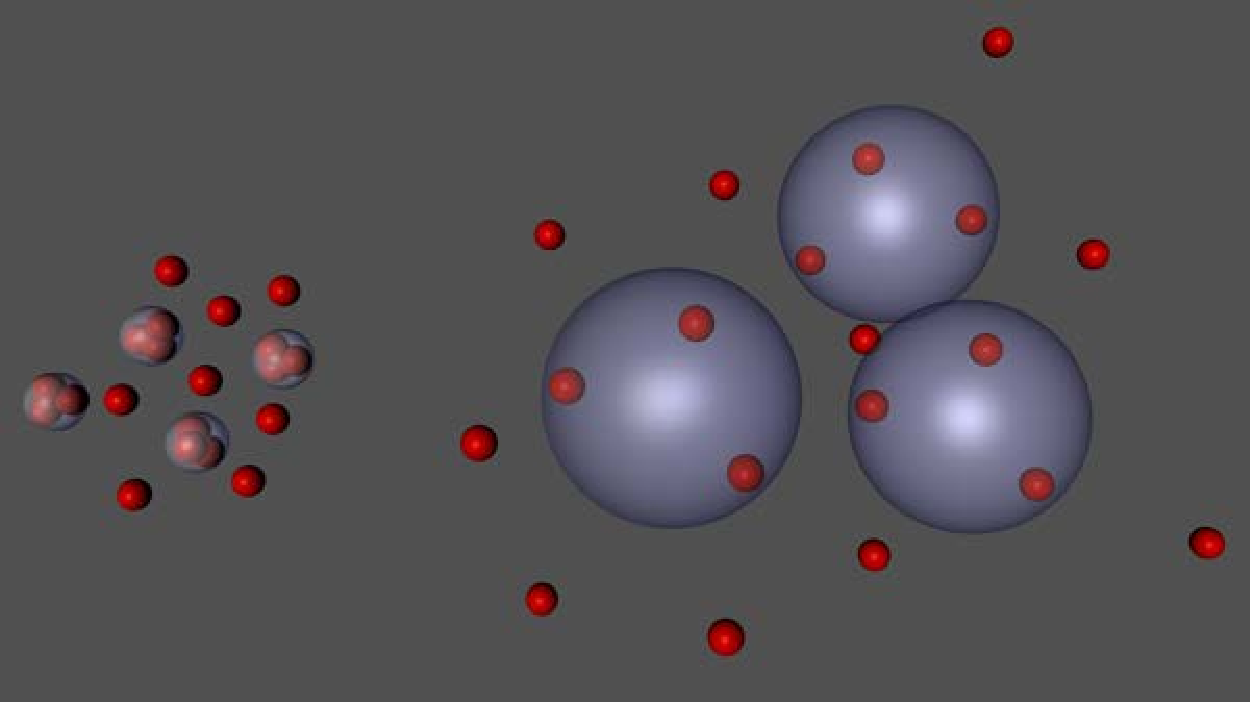
\includegraphics[width=0.6\textwidth]{Figures/efimov_scaling}
		\caption{Depiction of the scaling between successive Efimov states (blue spheres) in a ultracold atomic gas of Cs (red balls). Note that the scaling between the size of the Efimov states has been reduced from 22.7 for clarity.  Adapted from \cite{Modungo2014}.}
		\label{fig:efimov_cartoon}
	\end{figure}
%**************************************************************************************
\section{Cold Collisions}
Efimov's scenario would probably have remained a fairytale if not for crucial advancements that occurred in the field of ultracold atoms.  The driving force in the field was a race to achieve Bose-Einstein condensation, which was accomplished in 1995 \cite{Anderson1995}\cite{Bradley1995}\cite{Davis1995}.  A consequence of this push was that it became possible to not only achieve temperatures on the nK scale but it also became possible to tune the interactions in an atomic gas.  How this tunability becomes manifest through scattering is the focus of this section.
	\subsection{Scattering Principles}
	Let us briefly review some of the salient concepts of two-body quantum mechanical scattering.  Consider the case of two atoms of mass $m$ interacting through a potential  $V(|\mathbf{r}_1-\mathbf{r}_2|)$ which depends on the relative distance between atoms.  In this case the center of mass moves as a free particle of mass $2m$.  The interesting dynamics arise from the relative motion between atoms, which can be viewed as the scattering of a particle with reduced mass $\mu=m/2$ by the potential $V(\mathbf{r})$, where $\mathbf{r}$ is the relative position.
	
	This situation can be described by a stationary wavefunction $\psi_{\mathbf{k}}(\mathbf{r})$ which satisfies 
	\begin{equation}\label{eq:schroed}
		\bigg(-\frac{\hbar^{2}}{2\mu}\nabla^{2}+V(\mathbf{r})\bigg)\psi_{\mathbf{k}}(\mathbf{r})=E_{k}\psi_{\mathbf{k}}(\mathbf{r})
	\end{equation}
	where $E_{k}=\hbar^{2}k^{2}/2\mu$ is the collisional energy.  We seek scattering solutions with $E_{k}>0$ of the form $\ket{\psi}=\ket{\psi_{inc}}+\ket{\psi_{scat}}$, where $\ket{\psi_{inc}}$ is an incident wavepacket and $\ket{\psi_{scat}}$ is the scattered wave packet.  If we assume that the incident wavepacket is a plane wave of the form $\psi_{inc}(\mathbf{r})=e^{i\mathbf{k}\cdot\mathbf{r}}$, then the asymptotic form of $\psi_{\mathbf{k}}$ at large distances is given by 
	\begin{equation}\label{eq:scattering_wavefnc}
		\psi_{\mathbf{k}}(\mathbf{r})=e^{i\mathbf{k}\cdot\mathbf{r}}+f(k,\theta)\frac{e^{ikr}}{r}
	\end{equation}
	where $\theta$ is the scattering angle.  This asymptotic form tacitly assumes that the interaction potential is short range in the sense that $r^{2}V(\mathbf{r})\xrightarrow{r\rightarrow\infty}0$ and that $|\mathbf{r}|\gg\ell$, where $\ell$ is the range of the potential.  The factor $f(k,\theta)$ is the scattering amplitude, and from it the differential and total cross sections can be defined
	\begin{equation}\label{eq:cross_sections}
		\frac{\mathrm{d}\sigma}{\mathrm{d}\Omega}=|f(k,\theta)|^{2} \qquad \sigma_{tot}=\int|f(k,\theta)|^{2}\mathrm{d}\Omega
	\end{equation}
	
	A convenient way to characterize the scattering amplitude is through the partial-wave expansion which resolves $f(k,\theta)$ into contributions from different angular momentum states.  This expansion is given by
	\begin{equation}\label{eq:partial_wave_expansion}
		f(k,\theta)=\sum\limits_{l=0}^{\infty}\frac{2l+1}{k\cot{\delta_{l}(k)}-ik}P_{l}(\cos\theta)
	\end{equation}
	where $P_{l}(\cos\theta)$ are the Legendre polynomials, and $\delta_{l}(k)$ are the phase shifts of the outgoing partial waves with respect to the incoming ones.  For scattering of identical bosons (fermions) only even (odd) partial waves contribute.  This expansion is particularly convenient for collisions in cold atomic gases because s-wave scattering ($l=0$) dominates and higher partial waves can be neglected.  The physical reason for this is because the centrifugal potential $\hbar^{2}l(l+1)/2\mu r^{2}$ gives rise to a potential barrier, and for the case of the van der Waals potential ($V(r)=-C_{6}/r^{6}$) between Cs atoms, the potential barrier is $E/k_{B}=37\mu K$, $191\mu K$, $540\mu K$, and $1170\mu K$ for $l=1,2,3,4$ \cite{Chin2001}.  Since the relevant temperatures in the experiments confirming the existence of Efimov states reach a few $nK$ \cite{Huang2014}, higher partial waves will be reflected by the centifugal barrier.  Furthermore, the partial wave phase shifts $\delta_{l}(k)$ approach zero as $k^{2l+1}$ for low energy collisions ($k\rightarrow 0$).  This fact, combined with the strength of the higher $l$ centrifugal barriers, mean that elastic collisions between bosons in an ultracold gas is completely characterized by  the s-wave phase shift $\delta_{0}(k)$.

	At sufficiently low energies ($k\rightarrow 0$), the s-wave phase shift can be expanded in powers of $k$ in the \textit{effective range expansion} \cite{Chin2001}\cite{landau1977quantum}, and keeping only the first term results in
	\begin{equation}\label{eq:scattering_length_defined}
		k\cot\delta_{0}(k)=-\frac{1}{a}.
	\end{equation}
	The parameter $a$ is the s-wave scattering length,\footnote{Unless otherwise stated, the scattering length referred to in this paper is the s-wave scattering length.} and it is of extreme importance for low energy collisions because it completely characterizes the interaction.  In Fig. \ref{fig:scattering_length}, the relationship between the scattering length and the phase shift is shown.  For attractive potentials, the phase shift is positive and the scattering length is negative.  In very loose terms this can be interpreted as the potential ``pulling in" the scattered wave with respect to the unscattered wave.  For repulsive potentials, the phase shift is negative and the scattering length is positive.  Again, in very loose terms, this can be interpreted as the potential ``pushing out" the scattered wave.  It is worth emphasizing that this discussion is only for low energy scattering where $k\rightarrow 0$.
	
		%\begin{comment}
		\begin{figure}
			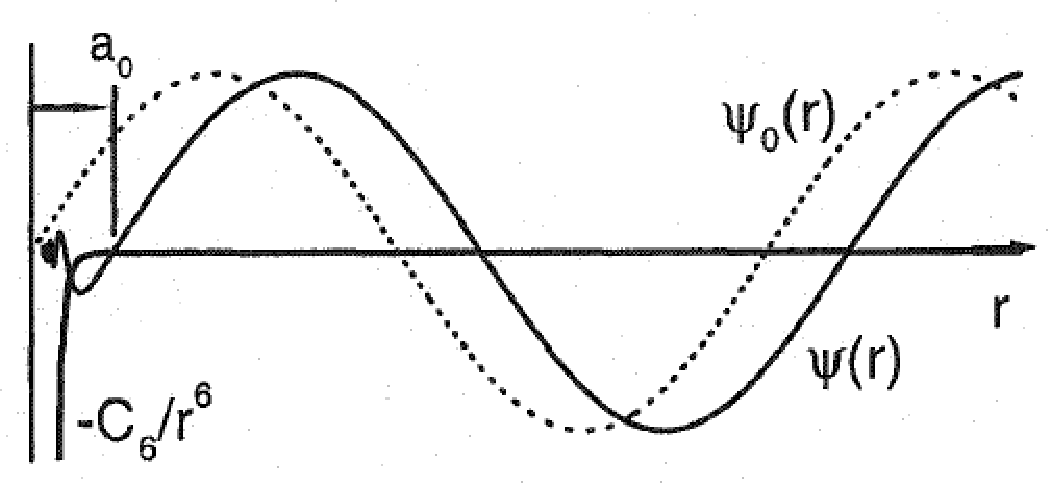
\includegraphics[width=0.6\textwidth]{Figures/scattering_length_with_C6}
			\caption{Depiction of the relation between the scattering length and the phase shift.  The unscattered wave is represented by $\psi_{0}(r)$ and the scattered wave is represented by $\psi(r)$.  The scattering length is positive and denoted by $a_{0}$.  Also shown is the van der Waals potential and the fast oscillations which occur in the interaction region.  Adapted from \cite{Chin2001}.}
			\label{fig:scattering_length}
		\end{figure}
		%\end{comment}
		
	The scattering length is also connected to the elastic cross section by the relation \cite{Dalibard1999}
	\begin{equation}\label{eq:cross_section}
		\sigma_{0}(k)=\frac{8\pi a^{2}}{1+k^{2}a^{2}},
	\end{equation}
	which leads to two asymptotic results
	\begin{eqnarray}
			\sigma_{0}(k) & = & 8\pi a^{2} \qquad \text{for } ka\ll 1\\
			\sigma_{0}(k) & = & 8\pi/k^{2} \qquad \text{for } ka\gg 1.
	\end{eqnarray}
	The second equation for $ka\gg 1$ represents the so-called \textit{unitary limit}, where the cross section reaches its maximum value.
	
	\subsection{Universal Dimer}
	As will be seen in later sections, Efimov trimer states exists in the resonant limit where the scattering length has been fine tuned such that $|a|\gg\ell$, where $\ell$ is the range of the interaction potential.  In this region, the particular  interaction can be considered as a perturbation on the general behavior which is set by the scattering length.  The properties of states in this region are referred to as \textit{universal} because they apply equally well to other short range potentials which produce the same scattering length.
	
	These unusual properties can be seen in two body scattering when the scattering length is large, $a\gg\ell$, and positive.  Physically, this corresponds to the case of the potential supporting a (real) bound state just below the scattering threshold \cite{Chin2010}\cite{Kohler2006}.  By solving Schr\"odinger's equation for this case, one finds that there is a shallow bound state of binding energy
	\begin{equation}\label{eq:halo_dimer_binding energy}
		E_{b}=\frac{\hbar^{2}}{2\mu a^{2}}.
	\end{equation}
	This is a bound state of the two-body system, and is thus a dimer.  More specifically, this state is referred to as a universal halo dimer.  The halo character can be seen from the wavefunction, given by 
	\begin{equation}\label{eq:halo_dimer_wvfnc}
		\psi(r)=\frac{1}{\sqrt{2\pi a}}e^{-r/a}.
	\end{equation}
	The radial probability of this state is then $\sqrt{\langle r^{2}\rangle}=a/\sqrt{2}$, and since we have assumed $a\gg\ell$ this corresponds to a bound state which has the bulk of its probability distribution beyond the range of the potential.
	
	\subsection{Feshbach Resonances}
	For a typical short range potential, the scattering length is usually close to the range of the potential in magnitude.  This statement can be thought of probabilistically because only by fine tuning of some parameters in the interaction to a specific value gives rise to a scattering length that is much larger in magnitude than the range \cite{Braaten_2006}.  In order to observe Efimov states it is necessary to able to tune the interaction such that the scattering length can be brought to the limit of $a\rightarrow\pm\infty$.  This is accomplished by taking advantage of resonant scattering.
	
	In general, a scattering resonance occurs when a bound state (real or virtual) is close to the scattering energy.  One possibility is for the bound state to be in the same potential as the one which is governing the scattering interaction.  By adjusting the depth or range (i.e. the shape of the potential) one is able to tune the position of the bound state relative to the scattering energy.  This is termed a \textit{shape resonance}.
	
	Another possibility is for the bound state to occur in another scattering channel.  This is known as a Feschbach resonance, which was first described independently by Herman Feshbach \cite{Feshbach1958}\cite{Feshbach1962} and Ugo Fano \cite{Fano1961}. To understand the concept of a scattering channel, consider two asymptotically separated atoms.  In this scenario each atom is described by its own internal quantum numbers $\ket{q_{1}}$ and $\ket{q_{2}}$.  The scattering potential\footnote{For the case of ultracold atomic collisions these are the Born-Oppenheimer potentials.} which connects these two states is referred to as a scattering channel and has eigenstates labeled by $\ket{\{q_{1},q_{2}\}}$.  The channel energy is given by the internal energy of the separated atoms, $E_{\alpha}=E(q_{1})+E(q_{2})$, and the total energy is $E_{tot}=E_{\alpha}+E$, where $E$ is the relative kinetic energy of the atoms in channel $\alpha$.  A channel $\beta$ is considered \textit{open} if the asymptotic states which it connects to have an energy that is below the scattering energy, $E_{\beta}\le E_{tot}$.  Likewise, the channel $\beta$ is considered \textit{closed} if the energy it asymptotically connects to is above the scattering energy, $E_{\beta}>E_{tot}$.  A collision can produce atoms in open channels but not closed channels because they simply do not have enough energy to form the separated atoms which label the closed channel.  However, in the presence of even a weak coupling between closed and open channels a resonance can occur \cite{Chin2010}.
	
	%\begin{comment}}
	\begin{figure}
		\centering
		\begin{subfigure}[b]{0.45\textwidth}
			\caption{}
			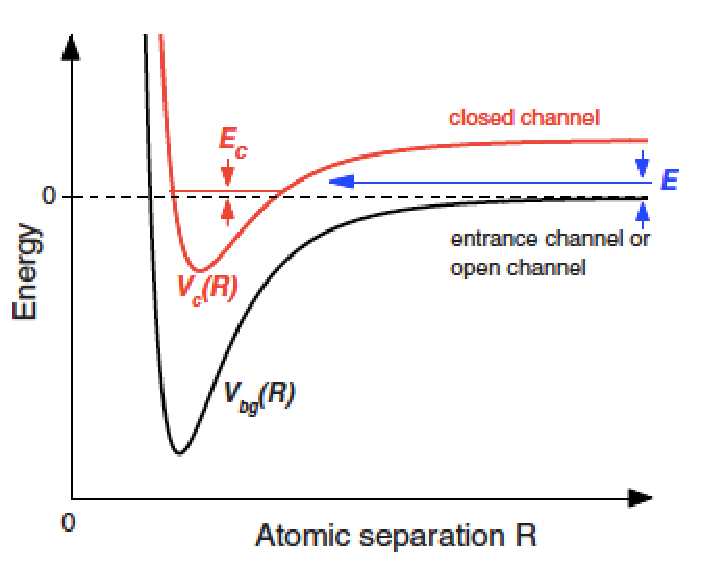
\includegraphics[width=\textwidth]{Figures/channels_defined}
			\label{fig:channel_defined}
		\end{subfigure}
		\begin{subfigure}[b]{0.45\textwidth}
			\caption{}
			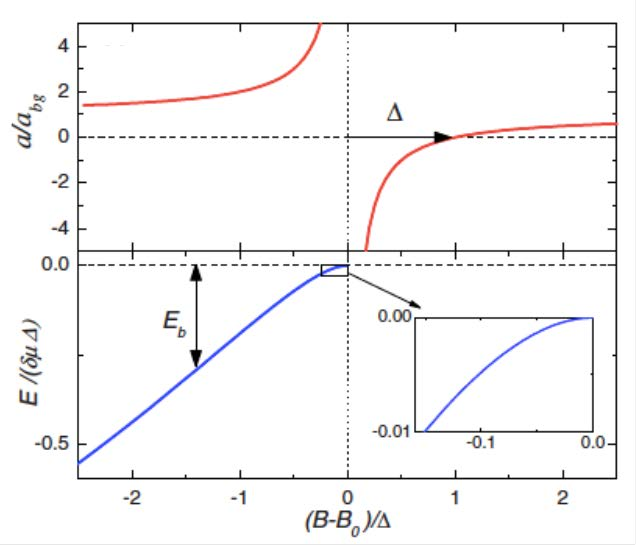
\includegraphics[width=\textwidth]{Figures/Resonances}
			\label{fig:resonance}
		\end{subfigure}
		\caption{(a) Two-channel model for Feshbach resonance.  Incident atoms in the entrance channel (the open channel) couple to a bound state of energy $E_{c}$ supported by the closed channel.  Since collisions take place for $E\rightarrow 0$, tuning $E_{c}$ to 0 allows for the resonant coupling to occur. (b) Scattering length near a resonance where a bound state crosses the scattering threshold. Inset shows the quadratic behavior of the binding energy near the resonance.  Adapted from \cite{Chin2010}.}
	\end{figure}
	%\end{comment}
	
	To see how this comes about, consider a two channel model, as depicted in Fig. \ref{fig:channel_defined}.  The channel potential $V_{bg}(R)$ is defined as the one which asymptotically connects to the energy of the separated atoms in the gas.  Since we are assuming these collisions are taking place in an ultracold gas, the relative kinetic energy $E$ is small, and the $V_{bg}$ is an open channel.  There is also another channel represented by the potential $V_{c}(R)$ which is a closed channel, and it is assumed to support a bound state $E_{c}$ near the threshold of the open channel.  If there is a difference in the magnetic moments $\delta\mu$ of the two channels, then in the presence of a magnetic field it is possible to tune the separation between $E_{c}$ and the threshold of the open channel.  Now, the only way for the atoms to "see" the bound state is in the presence of coupling $W(R)$ between the channels.  If the magnetic field at which the resonance occurs is $B_{0}$, then in the vicinity of $B_{0}$ the scattering length can be described by
	\begin{equation}\label{eq:a(b)}
		a(B)=a_{bg}\bigg(1-\frac{\Delta}{B-B_{0}}\bigg)
	\end{equation}
	where $\Delta=\Gamma_{0}/\delta\mu$ is the resonance width, $\Gamma_{0}=2\pi|\bra{E_{c}}W(R)\ket{E}|^{2}$ is the coupling strength, and $a_{bg}$ is the scattering length away from resonance.  This behavior is plotted in Fig. \ref{fig:resonance}.  In general, $\Delta$, $a_{bg}$, and $B_{0}$ can take on negative values.  For the case depicted in Fig. \ref{fig:channel_defined} and \ref{fig:resonance}, the bound state  $E_{c}$ begins below the scattering energy, and as the magnetic field is ramped higher it approaches $E$.  As this happens the scattering length begins approaching large positive values until the resonant magnetic field is reached where it jumps discontinuously  to large negative values.  This corresponds to $E_{c}$ being just above the scattering energy.  The importance of a Feshbach resonance of this type is that it enables a tunability of the scattering length over the entire range of $a\rightarrow\pm\infty$ by controlling an external parameter, the magnetic field.  This tunability is what enables observation of Efimov states in ultracold atomic gases \cite{Kraemer2006_1st_observ}\cite{Huang2014}.
	
	Not all Feshbach resonances are created equal, and a way to characterize them is in terms of which channel dominates the interaction.  For entrance-channel dominated Feshbach resonances, the interaction can be accurately described in terms of a single channel even near the resonance.   The condition for this description to be accurate is given in terms of the dimensionless resonance strength parameter \cite{Chin2010}
	\begin{equation}\label{eq:s_res_defined}
		s_{res}=\frac{a_{bg}}{\overline{a}}\frac{\delta\mu\Delta}{\hbar^{2}/m\overline{a}^{2}}
	\end{equation}
	The term $\overline{a}$ is a mean scattering length \cite{Gribakin1993}.  For the simple model of a coupled channel scattering in a open finite square well and closed infinite square well, $\overline{a}$ gives the radius of the well, and for the case of the van der Waals potential $V(R)=-C_{6}/R^{6}$ it is close to the range $\ell_{vdW}=1/2(m C_{6}/\hbar^{2})^{1/4}$.  When $s_{res}\gg1$ the resonance is classified as a entrance-channel dominated resonance, and it is very well modeled by $a(B)$ defined by Eq. \ref{eq:a(b)}. \cite{Chin2010}  Generally, entrance-channel dominated resonances tend to be broad resonances, and they are particularly well suited for the study of Efimov physics because they allow for better experimental control over the scattering length.

	\subsection{Relevant Feshbach Resonances}
In this section, the specific interactions which are relevant for collisions in a cold atom gas are covered. Particular attention will be paid to the interactions which are relevant for an ultracold gas of $^{133}\text{Cs}$ atoms in a magnetic field and cooled to their ground state, which is $\ket{F=3,m_{F}=+3}$ where $F=I+J$ and $m_{F}$ is the projection along the field.  Cesium is an alkali-metal with an electronic configuration of [Xe]$6s^{1}$, and so it has a single valence electron with a ground state of $^{2}S_{1/2}$.\begin{comment}\footnote{Following the usual notation of $^{2S+1}L_{J}$}.\end{comment}  The nuclear spin of  $^{133}Cs$ is $I=7/2$.

\begin{comment}
The Hamiltonian which characterizes this situation can be split into two components, those describing the internal structure of the atoms $\mathcal{H}_{0}$ and the interaction between atoms $\mathcal{H}_{1,2}$.  In the case of two neutral atoms in their ground state the Hamiltonian can be written as \cite{Chin2001}
\begin{eqnarray}\label{eq:total_interaction_hamiltonian}
\mathcal{H} & = & \mathcal{H}_{0}+\mathcal{H}_{12}\\
\mathcal{H} _{0}& = & \mathcal{H}_{k}+\mathcal{H}_{\textbf{hfs}}+\mathcal{H}_{Z}\\
\mathcal{H}_{12} & = & \mathcal{H}_{vdW}+\mathcal{H}_{ex}+\mathcal{H}_{dd}
\end{eqnarray}
Each of these terms will be briefly discussed below.
\end{comment}

In the asymptotic case of separated atoms, the system is described by the relative kinetic energy given by $E=\hbar^{2}k^{2}/2\mu$, the hyperfine interaction, and the effect of the magnetic field.  For the ground state electron $^{2}S_{1/2}$, the hyperfine interaction is described by
	\begin{equation}\label{eq:hyperfine_hamiltonian}
	\mathcal{H}_{\textbf{hfs}} = A_{\textbf{hfs}}\mathbf{I}\cdot\mathbf{J}
	\end{equation}
where $\mathbf{I}$ is the nuclear spin and $\mathbf{J}=\mathbf{L}+\mathbf{S}$ is the total electron angular momentum. The hyperfine interaction lifts the degeneracy of the $^{2}S_{1/2}$ state and splits into two hyperfine levels labeled by the quantum number $F$ associated with $\mathbf{F}=\mathbf{I}+\mathbf{J}$.  Specifically, this splitting is between $F=3$ and $F=4$ for Cs where $I=7/2$ and $S=1/2$, and the energy splitting is $\Delta E/h=9.2\text{ GHz}$.

The effect of the magnetic field is given by the Hamiltonian
\begin{equation}\label{eq:zeeeman}
	\mathcal{H}_{Z} = \frac{\mu_{B}}{\hbar}[g_{L}\mathbf{L} + g_{S}\mathbf{S} + g_{I}\mathbf{I}]\cdot\mathbf{B}
\end{equation}
This has the effect of lifting the $2F+1$ degeneracy of the hyperfine states labeled by F.  For magnetic fields small enough that the energy splitting due to the magnetic field is small compared to the hyperfine splitting, the projection of $\mathbf{F}$ along the direction of the magnetic field, labeled $m_{F}$, is a good quantum number. If the magnetic field is oriented along the z-direction, then the levels split linearly according to
\begin{equation}
	\Delta E(F,m_{F})=\mu_{B}g_{F}m_{F}B_{z}
\end{equation}
where $g_{F}$ is the hyperfine $g$-factor.  The splitting in this region is referred to as the Zeeman effect, and can be seen in Fig. \ref{fig:Zeeman_splitting}. 

\begin{comment}
For higher magnetic fields, the energy splitting is not as simple, but it can be calculated using the Breit-Rabi formula \cite{BreitRabi1931}.  The effect is that as the field becomes stronger such that the shift from the field is close to the hyperfine splitting, then the spins couple more strongly to the field than to each other.  In this case, $m_{F}$ is no longer a good quantum number but the individual projections, $m_{J}=m_{S}$ and $m_{I}$, along the field are good quantum numbers.  However, for an electron in the $^{2}S_{1/2}$ state, the hyperfine splitting between $F=4$ and $F=3$ is large at 9.2 GHz, so the field at which this happens is beyond 1000 G which is also beyond the experimental region for the study of Efimov physics ($<1000$ G) \cite{Huang2014}.
\end{comment}

\begin{figure}
	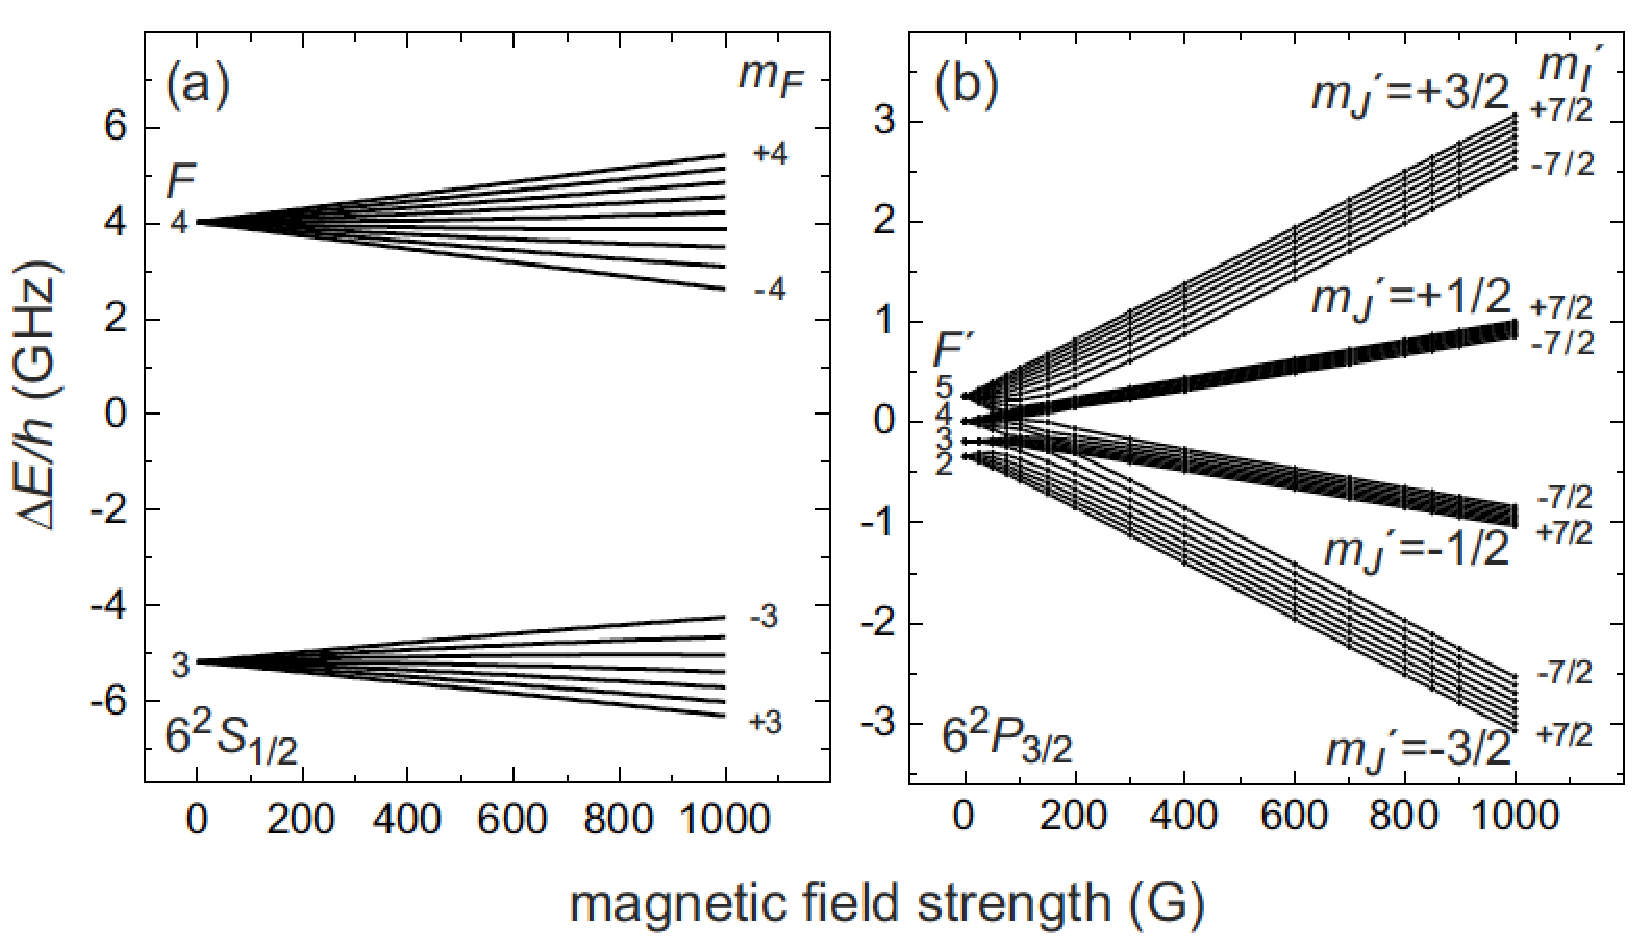
\includegraphics[width=0.6\textwidth]{Figures/Zeeman_splitting}
	\caption{Magnetic field dependence of ground state and excited state manifolds. (a) Ground state $^{2}S_{1/2}$ manifold for the experimentally relevant magnetic fields.  (b) Excited state $^{2}P_{3/2}$ manifold Adapted from \cite{Berninger2011}}
	\label{fig:Zeeman_splitting}
\end{figure}

For the excited state $^{2}P_{3/2}$, the hyperfine splitting is smaller than the ground state $^{2}S_{1/2}$ at $151$ MHz, $201$ MHz, and $251$ MHz between the hyperfine levels $F'=2,3,4,5$.  As a result, for the experimentally relevant region, the excited state manifold enters the Paschen-Back regime as the \textbf{IJ}-coupling breaks down \cite{Berninger2011_thesis}, where the good quantum numbers are given by the individual projections $m_{J}$ and $m_{I}$. This is because as the field becomes stronger such that the shift from the field is close to the hyperfine splitting, then the spins couple more strongly to the field than to each other.  This regime is reached at fields as low as 100 G, and the energy shifts are plotted in Fig. \ref{fig:Zeeman_splitting}.  These states are only used for imaging, as will be discussed later.

%\begin{comment}
\begin{figure}
	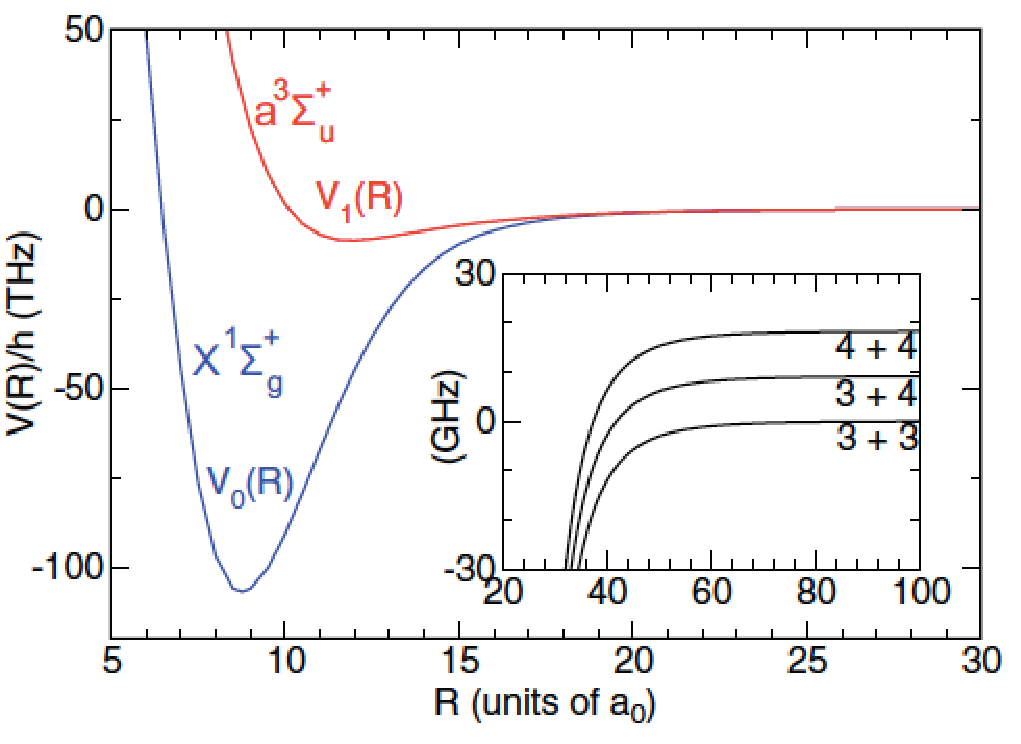
\includegraphics[width=0.5\textwidth]{Figures/Potential_curves}
	\caption{Molecular potential curves for singlet ($^{1}\Sigma^{+}_{g}$) and triplet states ($^{3}\Sigma^{+}_{u}$) of $\text{Cs}_{2}$.  The inset shows the long-range potentials separating to the hyperfine states $F=3$ and $F=4$, where the assumption is made that $B=0$.  Adapted from \cite{Hutson2008}}
	\label{fig:born_oppenheimer_pots}
\end{figure}
%\end{comment}

The previous analysis was for asymptotically separated atoms, now consider if we relax this condition and let them interact.  The van der Waals interaction is the dominant contribution, and physically arises from an induced electric dipole in the two atoms. The corresponding potential is given by $V(R)=-C_{6}/R^{6}$, where $C_{6}\approx 6890 E_{h} a_{0}^{6}$ for Cs. An important feature is that the van der Waals potential is isotropic and does not depend on the spin state of either atom.  It is the exchange interaction which adds the spin dependence at short range.  The exchange interaction is the result of the symmetrization required for the total wavefunction, and it is responsible for lowering (raising) the energy of the singlet (triplet) state, respectively.  The potentials including the van der Waals and exchange energy are plotted in Fig. \ref{fig:born_oppenheimer_pots}, \cite{Chin2010}\cite{Chin2001}.  These potentials support bound states, which are Cs dimers.   Since we are primarily interested in Feshbach resonances, the bound states of relevance are those which exist at the same energy as the two colliding atoms for a particular value of the magnetic field.  Thus, we are primarily interested in states which are close to dissociation and are bound by roughly less than $1$ GHz or less.  In this region, the states can be approximately described in terms of their atomic quantum numbers, molecular vibrational $n$, and their partial-wave angular momentum $\ell$.  Thus, the near threshold molecular states are reasonably well described by the set $n(F_{1}F_{2})f\ell(m_{f})$, where $f$ is the resultant of $F_{1}$ and $F_{2}$ and its projection is $m_{f}$.  

The colliding atoms are assumed to be in the state $\ket{F=3,m_{F}=3}$ and this sets the entrance channel.  For s-wave scattering the projection of the total angular momentum $m_{tot}=m_{f}+m_{\ell}=6$ is a conserved quantity.  As the magnetic field is changed, states with different magnetic moments from the colliding atoms $\ket{F=3,m_{F}=3}$ can cross the threshold, and if $m_{tot}=6$, then they can produce a Feshbach resonance.  There are two relevant states for the experiment done by the Grimm group, $-6(34)6d(6)$ and $-6(34)6s(6)$ which cross at fields of 820 G and 782 G.  The scattering length in this region is plotted in Fig. \ref{fig:a_vs_B_M2012}, and was obtained by the numerical model referred to as M2012 \cite{Berninger2013}.  This provides the mapping between the experimental control, the magnetic field, and the scattering length.  

\begin{comment}
The dipolar interactions $H_{dd}$ which are relevant are the spin-spin dipole interaction \cite{Stoof1988} and second-order spin orbit interaction \cite{Leo2000}\cite{Kotochigova2000}.  These terms have the same spin dependence, but their dependence on the interatomic separation is very different due to their different physical origins.  The spin-spin dipole is proportional to $-\alpha^{2}/R^{3}$ and the second-order spin orbit falls off exponentially because it depends on the wavefunction overlap \cite{Chin2010}.  The spin dependence of both interactions is the same, and is described by $V(r,\mathbf{S}_{1},\mathbf{S_{2}})=V(r)(\mathbf{S}_{1}\cdot\mathbf{S}_{2}-3(\mathbf{S}_{1}\cdot\hat{u})(\mathbf{S}_{2}\cdot\hat{u}))$, where $\hat{u}$ is the internuclear axis.

These interactions allow for two colliding atoms to change both their internal states and their relative angular moment state.  Thus, they allow for coupling of certain molecular states to the scattering threshold of the colliding molecules.  The quantum numbers describing the molecular states are $f$, $l$, $m_{f}$, and $m_{l}$, which are the total internal angular momentum given by $\mathbf{f}=\mathbf{F}_{1}+\mathbf{F}_{2}$, the rotational angular momentum, and their respective projections along the magnetic field.  It is the  dipolar interactions which allow for coupling to the scattering state of two atoms in the $F=3$ and $m_{F}=3$ state.  

Using these interactions, it is possible to numerically map out the position of the Feshbach resonances as a function of magnetic field \cite{Berninger2013}.  This provides the mapping between the experimental control provided by the magnetic field and the theoretically relevant parameter, the scattering length.  The two main Feshbach resonances of importance occur at fields of $782.97$G and at $820.26$G.  These resonances can be assigned to molecular potentials given by $f=6,l=0,m_{f}=6,m_{l}=0$ and $f=6,l=2,m_{f}=6,m_{l}=0$, respectively, and both are associated with the open entrance channel given by $F=3$ and $F=4$ (see inset in Fig. \ref{fig:born_oppenheimer_pots}).  The scattering length associated with these resonances are plotted in Fig. \ref{fig:a_vs_B_M2012}.  It is this region in which the Grimm group searched for the second Efimov state.
\end{comment}

\begin{figure}
	\centering
	\begin{subfigure}[b]{0.45\textwidth}
		\caption{}
		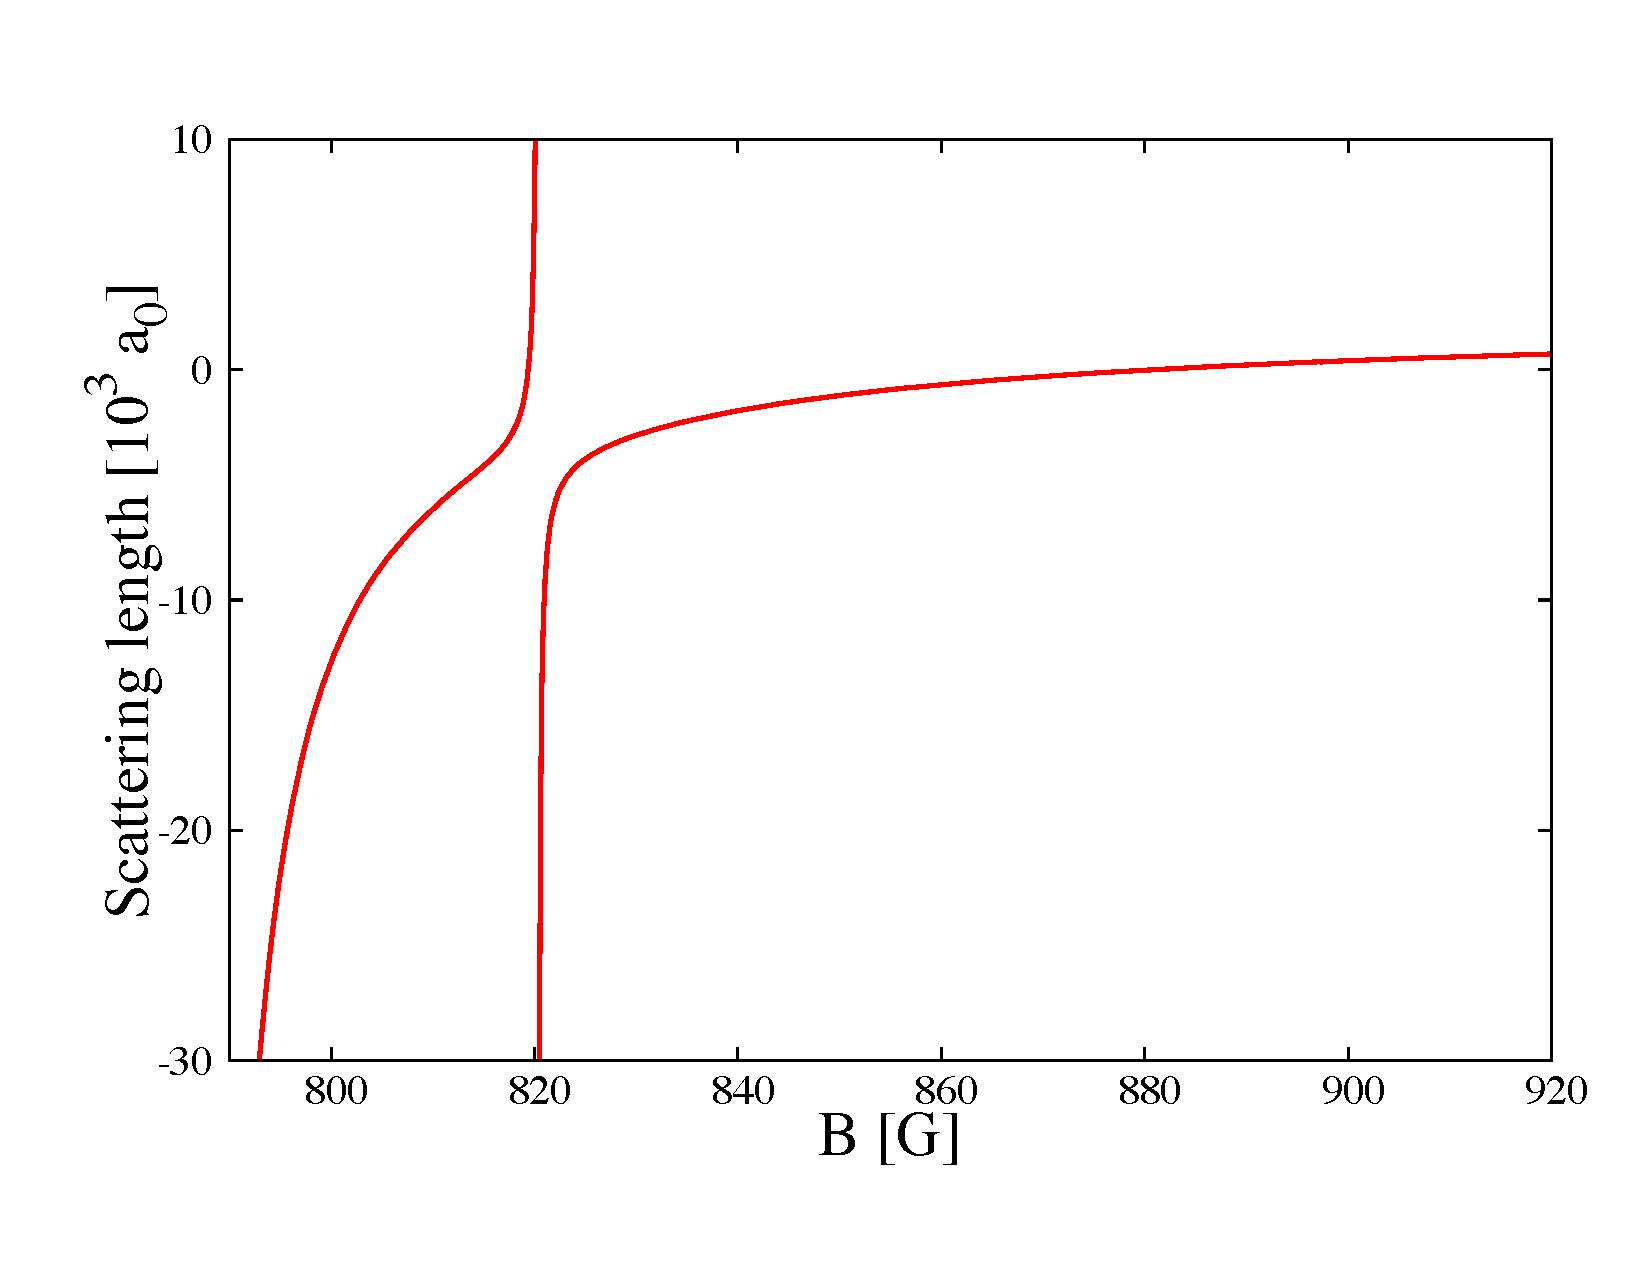
\includegraphics[width=\textwidth]{Figures/a_vs_B_M2012_2}
		\label{fig:a_vs_B_M2012}
	\end{subfigure}
	\begin{subfigure}[b]{0.45\textwidth}
		\caption{}
		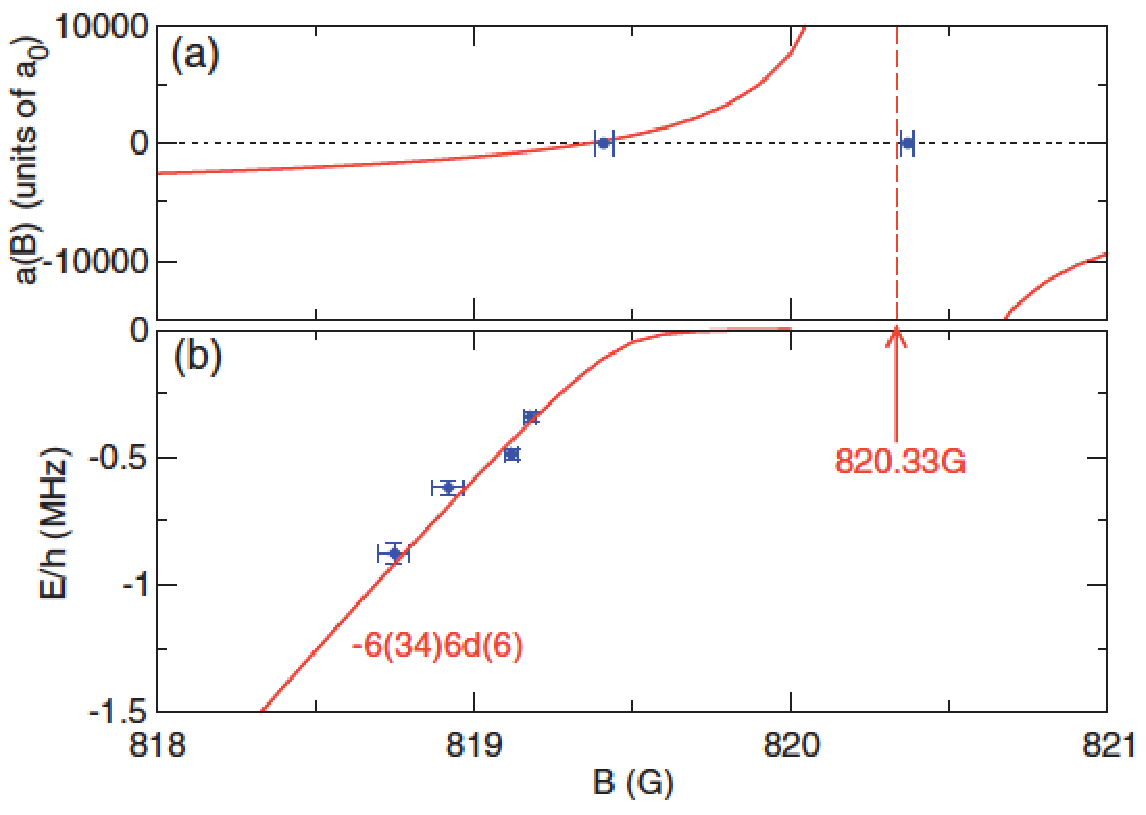
\includegraphics[width=\textwidth]{Figures/Feshbach_crossing}
		\label{fig:feshbach_crossing}
	\end{subfigure}
	\caption{(a) Scattering length vs magnetic field for an ultracold gas of Cs.  Shown here are the two relavant Feshbach resonances at 820.26G and 782.97G.  This is the region which is explored for the observation of Efimov states. (b) Example of where the $-6(34)6d(6)$ state crosses the threshold set by atoms in the $\ket{F=3,m_{F}=3}$ state.  Compare this to Fig. \ref{fig:resonance}. Plotted from data provided in \cite{Berninger2013}.}
	
\end{figure}

%\begin{comment}

%**************************************************************************************
\section{Efimov's Scenario}

\subsection{Hyperspherical Formalism}
In order to describe the Efimov effect and the associated states it is necessary to consider three mutually interacting atoms.  In general, Schr\"{o}dinger's equation is not analytically solvable for such a situation, however under certain conditions an exact solution can be obtained.  One such set of conditions leads to the Efimov effect which will be described below.

Consider three identical bosonic atoms of mass $m$ interacting through a potential $V(\mathbf{r}_{1},\mathbf{r}_{2},\mathbf{r}_{3})$.  The stationary wavefunction $\Psi(\mathbf{r}_{1},\mathbf{r}_{2},\mathbf{r}_{3})$ for such a system is given by the time-independent Schr\"{o}dinger equation
	\begin{equation}\label{eq:TISE}
		\bigg(-\frac{\hbar^{2}}{2m}\sum_{i}\nabla^{2}_{i} + V(\mathbf{r}_{1},\mathbf{r}_{2},
		\mathbf{r}_{3})\bigg)\Psi(\mathbf{r}_{1},\mathbf{r}_{2},
		\mathbf{r}_{3})=E\Psi(\mathbf{r}_{1},
		\mathbf{r}_{2},\mathbf{r}_{3})
	\end{equation}
For three atoms, there are nine independent coordinates, but if the potential is translationally invariant then the number of necessary coordinates can be reduced to six.  

A convenient way to represent these coordinates is to use the hyperspherical basis \cite{Braaten_2006}.  The hyperspherical coordinates are defined in terms of Jacobi coordinates.  For atoms of equal mass the Jacobi coordinates are given by
	\begin{equation}
		\mathbf{r}_{ij}=\mathbf{r}_{i}-\mathbf{r}_{j}, \qquad \mathbf{r}_{k,ij}=\mathbf{r}_{k}-\frac{1}
		{2}(\mathbf{r}_{i}+\mathbf{r}_{j})
	\end{equation}
where $(i,j,k)$ is a permutation of $(1,2,3)$.  Thus, there are three possible sets of Jacobi coordinates for a given three-body configuration.  An example one possible set is shown in Fig. \ref{fig:jacobi_coord}. 
	%\begin{comment}
	\begin{figure}[h]
		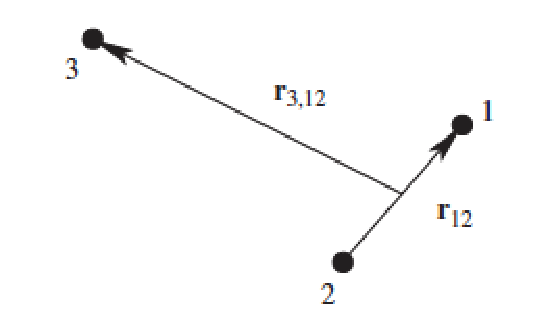
\includegraphics[width=0.3\textwidth]{Figures/hyperradial_coord}
		\caption{Example of one of the three possible Jacobi coordinates \cite{Braaten_2006}.}
		\label{fig:jacobi_coord}
	\end{figure}
	%\end{comment}
	
 Using the Jacobi coordinates the hyperradius
	\begin{equation}
		R^{2}=\frac{1}{3}(r^{2}_{12}+r^{2}_{23}+r^{2}_{31})=\frac{1}{2}r^{2}_{ij}+\frac{2}
		{3}r^{2}_{k,ij}
	\end{equation}
can be defined.  The hyperradius gives the separation of the three atoms. It is large if any atom is far from the other two, and it is small only if all three atoms are close together.

In addition to the hyperradius, a set of hyperangles can also be defined.  They are given by
	\begin{equation}\label{eq:hyperangle_def}
		\alpha_{k}=\arctan\bigg(\frac{\sqrt{3}r_{ij}}{2r_{k,ij}}\bigg)
	\end{equation}
where once again $(i,j,k)$ represent permutations of $(1,2,3)$.  An example of different three-body configurations with the same hyperradius but different hyperangle is shown in Fig. \ref{fig:hyperang_ex}.  The hyperangle $\alpha_{k}$ approaches a value of 0 when the atom labeled by $k$ is far from the other two atoms, and it approaches a value of $\frac{\pi}{2}$ when the $k$ atom approaches the center of mass of the other two atoms.  Also, for a given value of one of the hyperangles, say $\alpha_{k}$, then the other two hyperangles have a fixed range of possible values given by $|\frac{\pi}{3}-\alpha_{k}|<\alpha_{i}<\frac{\pi}{2}-|\frac{\pi}{6}-\alpha_{k}|$ \cite{Braaten_2006}.

	%\begin{comment}
	\begin{figure}[h]
		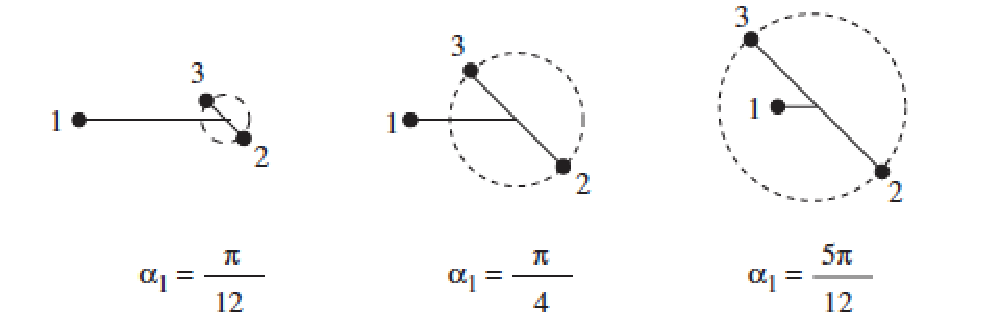
\includegraphics[width=0.6\textwidth]{Figures/hyperangular_example}
		\caption{Shown above are configurations that have the same hyperradius $R$, but for
			 different hyperangles: $\alpha_{1}=\frac{\pi}{12},\frac{\pi}{4},\frac{5\pi}{12}$.  If atoms 2 and 3 remain on the dashed circle, then the hyperradius R and hyperangle $\alpha_{1}$ will remain the same \cite{Braaten_2006}.}
		\label{fig:hyperang_ex}
	\end{figure}
	%\end{comment}
Using the hyperspherical coordinates, Schr\"{o}dinger's equation, Eq. \ref{eq:TISE}, can be written as
	\begin{equation}\label{eq:TISE_hyp}
		\bigg(T_{R}+T_{\alpha_{k}}+\frac{\Lambda^{2}_{k,ij}}{2mR^{2}}+V(R,\Omega)\bigg)
		\Psi(R,\Omega)=E\Psi(R,\Omega)
	\end{equation}
where $T_{R}$ and $T_{\alpha_{k}}$ are the kinetic energy operators associated with the hyperradius and hyperangle, respectively, and collective denoting $\Omega=(\alpha_{1},\alpha_{2},\alpha_{3}, \mathbf{\hat{r}}_{ij},\mathbf{\hat{r}}_{k,ij})$.  The generalized angular momentum term $\Lambda^{2}_{k,ij} $ acts as a centrifugal barrier, and can be ignored without loss of generality.\footnote{This assumption can be lifted, but doing so \textit{greatly} complicates the analysis without adding much physical insight. See \cite{Gasaneo2002} and \cite{Nielsen2001} for the general treatment including higher generalized angular momenta.}

It is possible to proceed using Schr\"{o}dinger's directly, but it is convenient to recast the problem in terms of a set of equivalent equations\footnote{They are equivalent, but spurious solutions can be generated where $\sum_{i}\psi^{(i)}=0$ when $\psi^{(i)}$ is non-trivial \cite{Braaten_2006}.}, known as the \textit{Faddeev equations}\cite{Faddeev1961}, which take advantage of an inherent symmetry in three-body problems.  This approach was first introduced by Fedorov and Jensen \cite{Fedorov1993}, and is followed closely herein.  The Faddeev equations are generated by looking for solutions to Eq. \ref{eq:TISE_hyp} of the form 
	\begin{equation}\label{eq:Faddeev_psi}
		\Psi(\mathbf{r}_{1},\mathbf{r}_{2},\mathbf{r}_{3})=\psi^{(1)}(\mathbf{R},\alpha_{1})+
		\psi^{(2)}(\mathbf{R},\alpha_{2})+\psi^{(3)}(\mathbf{R},\alpha_{3})
	\end{equation}
where the wavefunctions $\psi^{(i)}$ satisfy a set of equations given by
	\begin{equation}\label{eq:Faddeev_eqs}
		\big(T_{R}+T_{\alpha_{k}}\big)\psi^{(i)}+V\big(\sqrt{2}R\sin\alpha_{i}\big)\sum_{j=1}^{3}\psi^{(j)} = E\psi^{(i)}
	\end{equation}
where the potential has been expressed as a sum of pair-wise potentials $V(r_{ij})=V(\sqrt{2}R\sin\alpha_{k})$. The advantage of working with the Faddeev equations instead of Schr\"{o}dinger's equation directly can be seen by setting $\psi^{(2)}=\psi^{(3)}=0$.  In this limiting case, the Faddeev equations reduce to a two-body problem between atoms 2 and 3 described by the wave function $\psi^{(1)}$ \cite{Braaten_2006}.  Thus, the Faddeev equations are an excellent choice to describe a system that has inherently strong pairwise correlations, which is exactly the case in Efimov's scenario where the three-body problem is explored in the presence of a two-body resonance.

To further simplify the problem, it is possible to express the Faddeev equations (Eq. \ref{eq:Faddeev_eqs}) into a single integro-differential equation by averaging over $\psi^{(2)}$ and $\psi^{(3)}$.\footnote{By doing so, information about the exact three-body configuration is lost.} This yields the integro-differential equation
	\begin{equation}\label{eq:IntDiff_faddeev}
		\big(T_{R}+T_{\alpha}-E\big)\psi(R,\alpha)=-V(\sqrt{2}R\sin\alpha)\Bigg[\psi(R,\alpha)+\frac{4}{\sqrt{3}}\int\limits_{|\frac{\pi}{3}-\alpha|}^{\frac{\pi}{2}-|\frac{\pi}{6}-\alpha|}\mathrm{d}\alpha'\frac{\sin2\alpha'}{\sin2\alpha}\psi(R,\alpha')\Bigg]
	\end{equation}
Ostensibly, this might not appear to simplify the problem very much, but in going from Eq. \ref{eq:TISE} to Eq. \ref{eq:IntDiff_faddeev} we have been able to reduce the number of independent coordinates from six to two. Solutions to  Eq. \ref{eq:IntDiff_faddeev} can be obtained by expanding the wavefunction in a set of eigenfunctions
	\begin{equation}\label{eq:hyp_eigen_exp}
		\psi(R,\alpha)=\frac{1}{R^{5/2}\sin2\alpha}\sum_{n}f_{n}(R)\varphi_{n}(R,\alpha)
	\end{equation}
where $\varphi_{n}(R,\alpha)$ are solutions to the eigenvalue problem for a fixed value of $R$
 	\begin{equation}\label{eq:hyperangular_eigen_ODE}
 		-\frac{\partial^{2}\varphi_{n}}{\partial\alpha^{2}}+\frac{2mR^{2}}{\hbar^{2}}
 		V\big(\sqrt{2}R\sin\alpha\big)\Bigg[\varphi_{n}(R,\alpha)+\int\limits_{|\frac{\pi}{3}-\alpha|}^{\frac{\pi}{2}-|\frac{\pi}{6}-\alpha|}\mathrm{d}\alpha'\varphi_{n}(R,\alpha')\Bigg]=\lambda_{n}(R)\varphi_{n}(R,\alpha)
 	\end{equation}
 The corresponding channel eigenvalues $\lambda_{n}(R)$ depend parametrically on the hyperradius $R$ and define the channel potentials for the hyperradial wavefunctions.  Upon insertion of the expansion in Eq. \ref{eq:hyp_eigen_exp} into Eq. \ref{eq:IntDiff_faddeev} and projecting onto $\bra{\varphi_{n}}$ one can obtain the coupled differential equation for $f_{n}$.  However, if $\lambda_{n}(R)$ varies slowly with $R$, then the coupling terms $\bra{\varphi_{n}}\frac{\partial}{\partial R}\ket{\varphi_{m}}$ and $\bra{\varphi_{n}}\frac{\partial^{2}}{\partial R^{2}}\ket{\varphi_{m}}$ can be neglected.  This is known as the \textit{adiabatic hyperspherical approximation} \cite{Braaten_2006}\cite{Fedorov1993}, and is frequently made.  In this case the eigenvalue equation for the hyperradial wavefunctions is given by
 	\begin{equation}\label{eq:hyperrad_eigen_ODE}
 		-\frac{\hbar^{2}}{2m}\Bigg[\frac{\mathrm{d}^{2}}{\mathrm{d}R^{2}}+\underbrace{\frac{\lambda_{n}(R)-1/4}{R^{2}}}_{V_{n}(R)}
 		\Bigg]f_{n}(R)=Ef_{n}(R)
 	\end{equation}
 Depending on the value of the eigenvalues $\lambda_{n}(R)$, the potential $V_{n}(R)=(\lambda_{n}(R)-1/4)\frac{\hbar^{2}}{2m}$  can act as either an attractive or a repulsive potential.  It is this fact which gives rise to the Efimov effect, as will be shown in the next section.
 \subsection{Efimov Effect}
	Thus far, the main assumption that has been made in reformulating the three-body problem of Eq. \ref{eq:TISE} is that the three-body interaction potential can be expressed as a sum of pairwise potentials.\footnote{Which is to say that any true three-body term is at least negligible.}  Now, consider the case where those pairwise potentials are attractive and fall off faster than $r^{-2}$ where $r$ is the relative distance.  In this case, a characteristic length $\ell$ can be defined beyond which the potential can be taken to be zero.  When the scattering length and relative separation are beyond the characteristic length $\ell$ satisfy the relation $\ell\ll r \ll |a|$, then it is possible to solve the eigenvalue problem of Eq. \ref{eq:hyperangular_eigen_ODE} in appropriate regions.  By applying boundary conditions on the logarithmic derivative of the eigenfunctions $\varphi_{n}$ a transcendental equation for the eigenvalues can be obtained \cite{Efimov1971}\cite{Braaten_2006}\cite{Fedorov1993}
	\begin{equation}\label{eq:channel_eigenvalue_eq}
		\sqrt{\lambda}\cos\bigg(\frac{\pi}{6}\sqrt{\lambda}\bigg)=\frac{8}{\sqrt{3}}\sin\bigg(\frac{\pi}{6}\sqrt{\lambda}\bigg)+\sqrt{2}\frac{R}{a}\sin\bigg(\frac{\pi}{2}\sqrt{\lambda}\bigg)
	\end{equation}
	The first three solutions for $a<0$ and $a>0$ to this equation are plotted in Fig. \ref{fig:hyp_ang_eigenv}. As $R/|a|\rightarrow0$, all eigenvalues approach positive values except for the lowest eigenvalue which approaches a value of $\lambda_{0}=-1.01252=-s_{0}^{2}$.  
	
	The channel potentials associated with the channel eigenvalues are plotted in Fig. \ref{fig:hyper_potentials}.  The relationship comes from the potential term in Eq. \ref{eq:hyperrad_eigen_ODE}, and is defined by $V_{n}\propto\big(\lambda_{n}(R)-1/4\big)/R^{2}$, It can be seen from Fig. \ref{fig:hyper_potentials} that all eigenvalues give rise to a repulsive potential except for the lowest eigenvalue which is associated with an attractive potential.  In the limit of $R/|a|\rightarrow0$ the eigenvalue approaches the constant value of $-s_{0}^{2}$ which means that the potential in this region is $V_{0}\propto-1.2625/R^{2}$.  This type of a potential can support an infinite number of bound states, and the presence of this potential in the three-body spectrum is precisely what gives rise to the Efimov's effect \cite{Efimov1970}\cite{Efimov1971}.
	 %\begin{comment}
	  \begin{figure}
	  	\centering
		\begin{subfigure}[b]{0.45\textwidth}
			\caption{Channel Eigenvalues}
			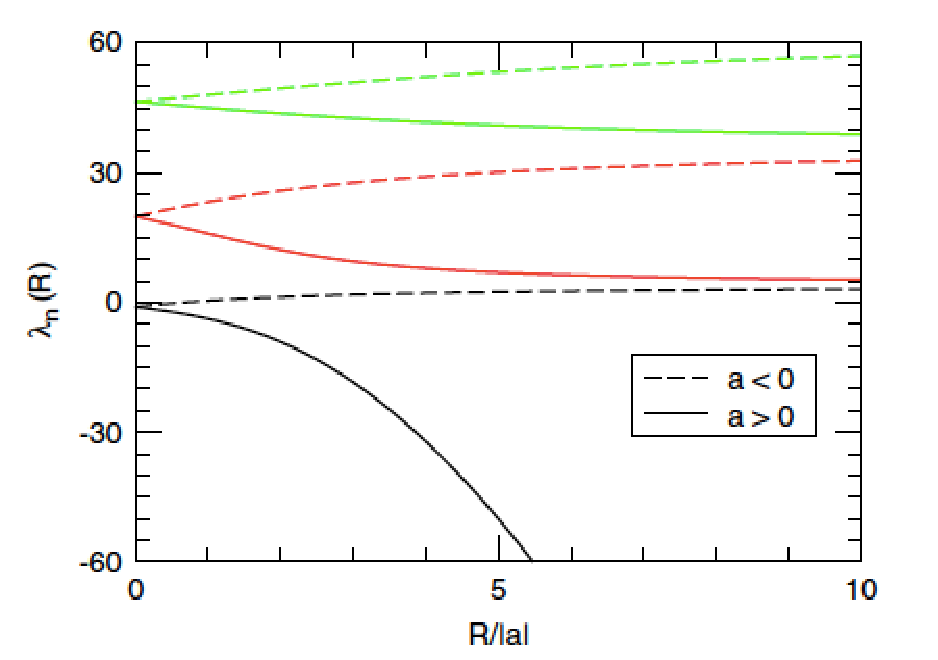
\includegraphics[width=\textwidth]{Figures/hyperangular_eigenvalues}
			\label{fig:hyp_ang_eigenv}
		\end{subfigure}
		\begin{subfigure}[b]{0.45\textwidth}
			\caption{Channel Potentials}
			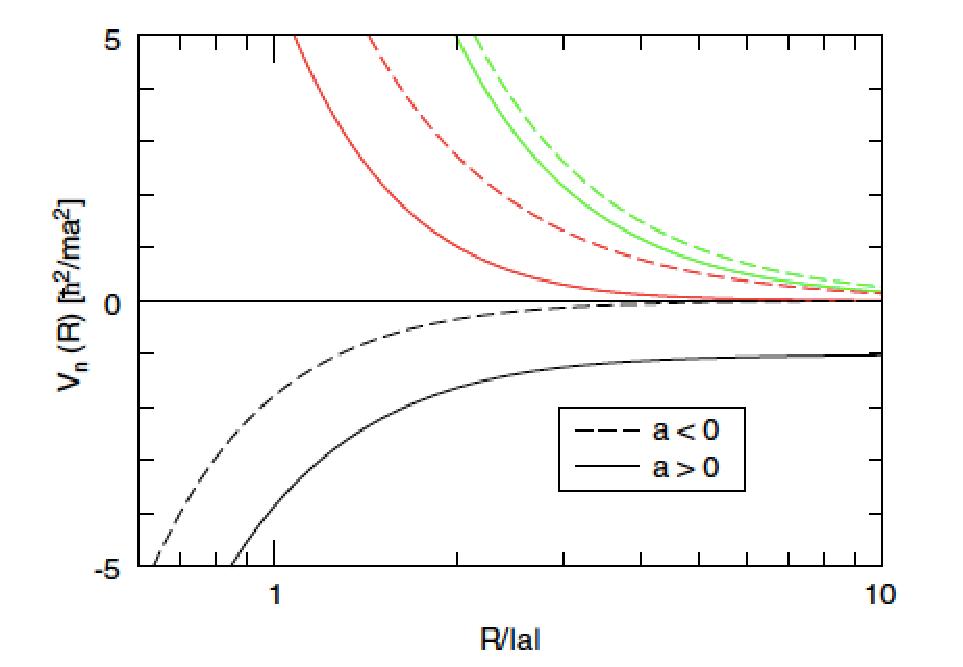
\includegraphics[width=\textwidth]{Figures/hyperradial_potentials}
			\label{fig:hyper_potentials}
		\end{subfigure}
		\caption{(a) First three hyperangular eigenvalues and (b) associated hyperradial channel potentials.  All channel potentials approach the three-atom scattering threshold as $R/|a|\rightarrow \infty$, except for the lowest channel potential for $a>0$.  In that case the potential approaches the atom-dimer threshold given by $-\hbar^{2}/m a$. Adapted from \cite{Braaten_2006}}
	\end{figure} 
	%\end{comment}
	
\subsection{Efimov States}

	As seen in the previous section, in the presence of a resonant two-body interaction the three-body system develops an attractive potential.  Consider the case of the so-called \textit{resonant limit} \cite{Braaten_2006} when $|a|\rightarrow \infty$.  The lowest channel eigenvalue approaches $\lambda_0=-s_0^2$, and the hyperradial wavefunction satisfies
	\begin{equation}
		-\frac{\hbar^{2}}{2\mu}\bigg[\frac{\mathrm{d}^{2}}{\mathrm{d}R^{2}}+\frac{s_0^2+1/4}{R^2}\bigg]f_0(R)=E f_0(R).
	\end{equation} 
	The normalizable solution to this equation is
		\begin{equation}\label{eq:f_0_resonant_limit}
			f_0(R)=N\sqrt{R}K_{is_0}(\kappa R)
		\end{equation}
	where N is some normalization, $K_{i s_{0}}$ is the modified Bessel function of the second kind, and $\kappa$ is the binding wavenumber defined related to the binding energy of an Efimov trimer $E_{T}=\hbar^{2}\kappa^{2}/m$.  The full wavefunction associated with this state can be written as
		\begin{equation}\label{eq:wavefunction_efimov_trimer}
			\Psi\big(\mathbf{r}_1,\mathbf{r}_2,\mathbf{r}_3\big)=\frac{f_{0}(R)}{R^{5/2}}\sum_{i=1}^{3}\frac{\sinh[s_0(\frac{\pi}{2}-\alpha_{i})]}{\sin(2\alpha_{i})}.
		\end{equation}

	In the limit of $\kappa R\ll 1$ the solution Eq. \ref{eq:f_0_resonant_limit} takes on the asymptotic form
		\begin{equation}\label{eq:asym_f0}
			f_0(R)\rightarrow \sqrt{\frac{\pi}{s_0 \sinh(\pi s_0)}}\sqrt{R}\sin(s_0\ln\kappa R+\alpha_0),
		\end{equation}
	where $\alpha_0$ is some universal phase.  This solution is strictly valid only in a region outside the range $\ell$ of the two-body potential.  However, by matching the solution we obtained in Eq. \ref{eq:asym_f0} by applying a boundary condition to a specific potential, it is possible to set the spectrum of binding energies.  The resulting spectrum is given by \cite{Efimov1970}\cite{Braaten_2006}
		\begin{equation}\label{eq:Efimov_trimer_binding_E}
			E_{T}^{(n)}=\big(e^{-2\pi/s_0}\big)^{n-n_{*}}\frac{\hbar^{2}\kappa_{*}^{2}}{m}
		\end{equation}
	where $\kappa_{*}$ is the binding wavenumber of the Efimov trimer labeled by $n_{*}$.  The parameter $\kappa_{*}$ is related to the so-called \textit{three-body parameter} which depends on the structural details of the two-body interaction and is found from the aforementioned boundary condition.
	
	There are several remarkable aspects of the Efimov spectrum given by Eq. \ref{eq:Efimov_trimer_binding_E}.  It is a geometric spectrum where successive states have relative binding energies given by the universal scaling $e^{-2\pi/s_{0}}\approx 1/515.7$.  Also, there are infinitely many states, and they have an accumulation point at $E_{T}^{(n\rightarrow\infty)}=0$. Furthermore, since all of the structure of the specific two-body interaction is contained within the three-body parameter and equivalently $\kappa_{*}$, this geometric scaling between three-body states is universal and independent of the character of the system.  This is precisely the reason why a problem formulated in the context of nuclear physics can be explored in ultracold atoms.
	
	Thus far, only the resonant limit corresponding to divergence of the scattering length has been considered.  This condition can be relaxed for finite values of the scattering length.  The result of such calculations \cite{Fedorov1993}\cite{Braaten_2006}\cite{Braaten2008}\cite{Nielsen2001} is that the attractive $-1/R^{2}$ potential is cut-off at $R\approx |a|$ and puts a bound on the number of states. For finite scattering length the number of states is given by $N\approx\frac{s_{0}}{\pi}\ln(|a|/\ell)$\cite{Efimov1970} \cite{Efimov1971}.
	
	\begin{comment}The number of states can be easily determined by counting the nodes in the hyperradial wavefunction \cite{Efimov1970}\cite{Efimov1971}. \end{comment}
	
	The salient results can be visualized in Fig. \ref{fig:efimov_scenario}, which is commonly referred to as Efimov's scenario \cite{Efimov1970}\cite{Ferlaino2011}\cite{Kraemer2006_1st_observ}. In this figure the energy spectrum of the universal dimer, Efimov trimer, and the three atom scattering states are depicted as a function of the inverse scattering length $1/a$.  A physical system has a particular value of the scattering length and corresponds to a vertical line.  In turn, tuning of the scattering length corresponds to sweeping of the vertical line along the abscissa. 
	
	The natural boundary for the three-body spectrum is given by the three-atom scattering threshold ($E=0$ for $a<0$) and the universal dimer \cite{landau1977quantum} threshold ($E=-\hbar^{2}/ma^{2}$ for $a>0$).  The subset of this region where $a<0$ is sometimes referred to as the \textit{Borromean region}, where the three-body Efimov states persist even though the two-body system is unbound.\footnote{Borromean refers to the Borromean rings.  They are a set of three rings connected in such a way that no two are linked, and if any one is removed then all three fall apart. The name of the rings refer to the Borromeo family.  They were an affluent Milanese family from the 15th century who first used the symbol of the three interconnected rings on their family crest.}  In this region, the Efimov states become unbound as they cross the three-atom scattering threshold at $E=0$.  The scattering length at which this happens for the $n$-th Efimov state is given by $a_{-}^{(n)}$.  At this scattering length, a low-energy collision between three atoms can resonantly couple to the Efimov trimer.  
	
	For the non-Borromean region, where $a>0$ and below the halo dimer binding energy, the Efimov states begin to couple to the atom-dimer threshold.  The scattering length at which this happens for the $n$-th Efimov state is labeled by $a_{*}^{(n)}$.  As the Efimov state approaches the atom-dimer threshold, it can be thought of as an Efimov state consisting of an atom and a dimer, whose size is given by the atom-dimer scattering length.  The crossing values of the scattering length for both regions obey the geometric scaling given by \cite{Braaten_2006}
		\begin{equation}\label{eq:geometric_scaling_a}
			\frac{a_{-}^{(n+1)}}{a_{-}^{(n)}}=\frac{a_{*}^{(n+1)}}{a_{*}^{(n)}}=e^{\pi/s_{0}}\approx22.7
		\end{equation} 
	and the relationship between the crossing values for the $n$-th Efimov state is  $a_{-}^{(n)}=-\frac{22.7}{1.06}a_{*}^{(n)}$.  The discrete scaling symmetry is a significant feature of Efimov's scenario and is confirmed by the experiment performed the Grimm group \cite{Huang2014}, as will be seen in a following section.
	
	%\begin{comment}
	\begin{figure}
		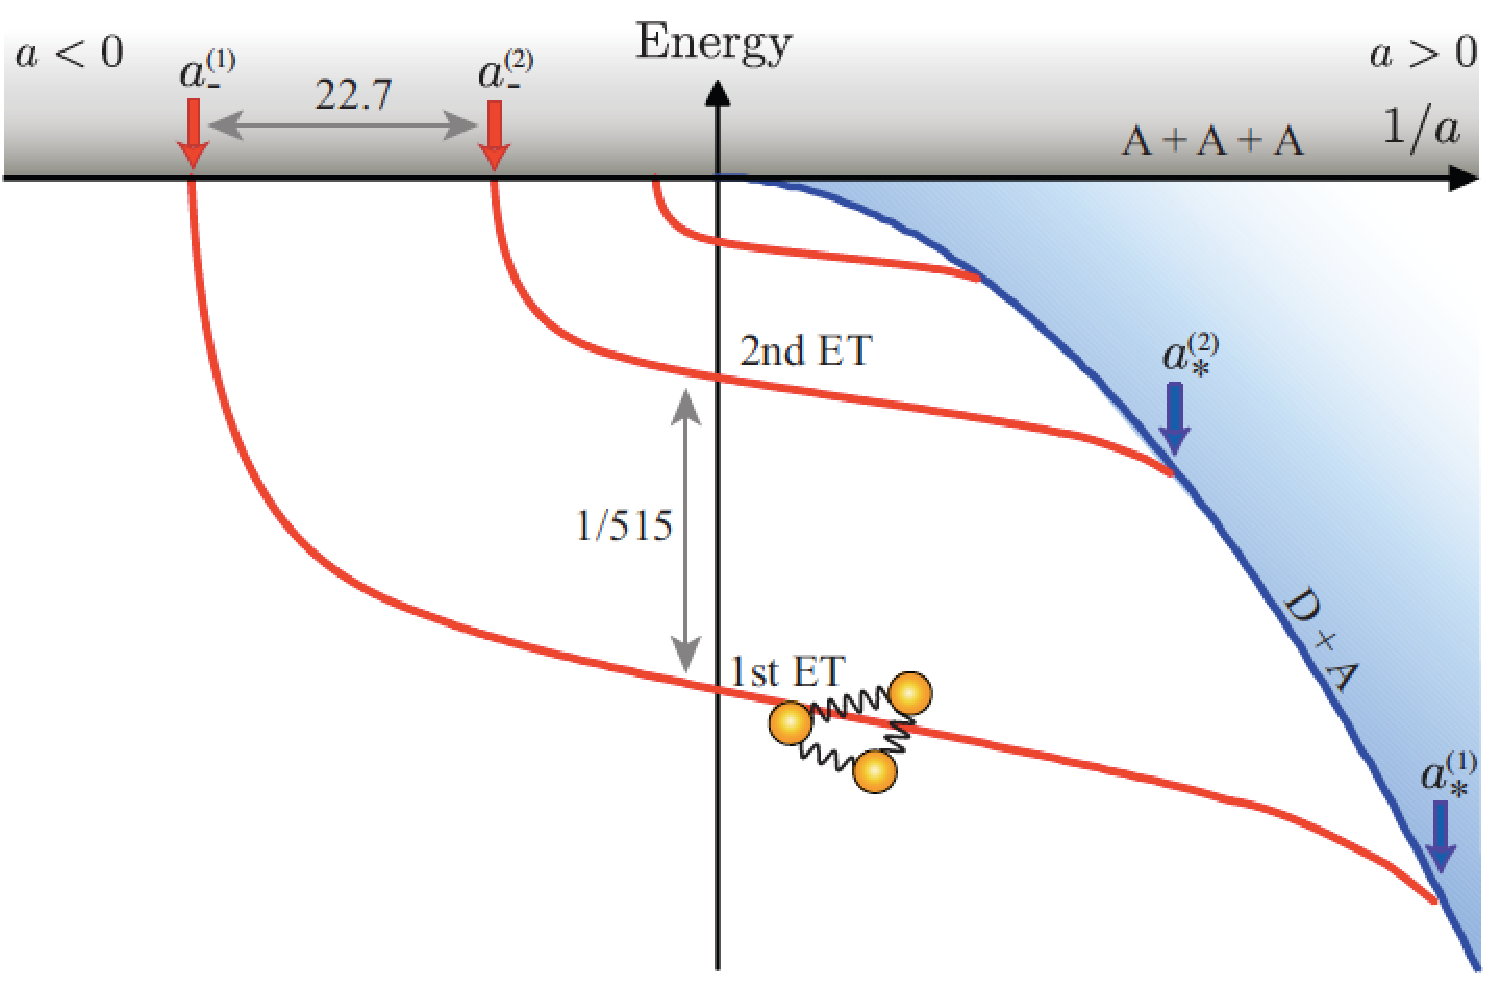
\includegraphics[width=0.75\textwidth]{Figures/efimov_phase_diagram}
		\caption{\textbf{Efimov's Scenario}.  This plot depicts the binding energy of successive Efimov states (red lines) as a function of $1/a$.  The triatomic scattering threshold is set to $E=0$ and is the grey region labeled by (A+A+A).  There also exists a universal dimer for $a>0$, whose binding energy sets the atom-dimer threshold labeled by (D+A).  The crossing values where the Efimov state becomes unbound is given by the red and blue arrows for the triatomic and atom-dimer thresholds, respectively.  The geometric scaling is reduced from 22.7 to 2 and only the first three states are shown. Adapted from \cite{Berninger2011}}
		\label{fig:efimov_scenario}
	\end{figure}
	%\end{comment}
%**************************************************************************************

\section{Three-body Recombination}
In ultracold atomic physics, Efimov states are revealed through their influence on collisions rather than direct observation.  Their influence manifests itself in three-body recombination processes.  These processes are described by a low-energy collision of three atoms $(A)$ which results in the formation of a bound dimer $(D)$ and an atom, $A+A+A \rightarrow D+A$.  These processes are a first step towards the association of molecules in an ultracold gas, and the creation of a cold molecular gas \cite{Jochim2003}.  They also place a limit on the lifetime of a trapped atomic cloud.

Recombination is typically discussed in terms of an event rate per unit time and volume, $\nu_{rec}=\alpha_{rec}n^{3}$, where $n$ is the particle density \cite{Weber2003_recomb}. The recombination rate constant $\alpha_{rec}$ in the low-energy limit follows a dependence of $\alpha_{rec}=C(a)\hbar a^{4}/m$ where the scaling with $a^{4}$ is universal \cite{Fedichev1996} and the dimensionless factor $C(a)$ contains all of the non-trivial physics \cite{Esry1999}\cite{Nielsen1999} and can be predicted by theory \cite{Braaten_2006}.

In a typical recombination process, the molecular binding energy $E_{b}$ is converted to kinetic energy.  If the recombination results in an atom and a dimer, then they would receive a kinetic energy of $E_{b}/3$ and $2E_{b}/3$, respectively.  Since the energy $E_{b}$ is usually large compared to the trapping potential, both the atom and the dimer escape the trap.  The experiment manifestation of this process is a decay in the density of the trapped atomic gas as a function of time, and for a three-body interaction this is described by the differential equation
	\begin{equation}\label{eq:3_body_recomination_equation}
		\frac{\mathrm{d}n(\mathbf{r},t)}{\mathrm{d}t}=-L_{3}n^{3}(\mathbf{r},t)
	\end{equation}
where $L_{3}$ is the three-body loss coefficient.  The relationship  between the three-body loss coefficient and the recombination rate constant $\alpha_{rec}$ is given by $L_{3}=n_{l}\alpha_{rec}$ where $n_{l}$ is the number of atoms lost from the trap.  Typically, the kinetic energy gained by both the atom and the dimer is enough to expel both from the trap, corresponding to $n_{l}=3$.  For the case considered in the experiment done by the Grimm group on Cs \cite{Huang2014}, the trapping potential is on the order of 10 $\mu\text{K}$, which corresponds to  few neV, and the deeply bound dimers have a binding energy of at least a few $\mu$eV.  \begin{comment}However,  due to the presence of the halo dimer for large positive scattering lengths, it is possible that the atom will remain trapped while the dimer will escape.  In this case $n_{l}=2$.  It is also possible that the dimer can stay trapped in the cloud.  The dimer will then quickly quench its high vibrational excitation in another collision with an atom in the cloud. \cite{Weber2003_recomb}. These collisions typically release enough energy that the collision participants are expelled. In all cases described above, recombination gives rise to heating. \cite{Weber2003_recomb}\cite{Huang2014}\cite{Rem2013}. \end{comment} 

The dependence of the three-body loss coefficient on scattering length reveals the connection between recombination processes and Efimov states.  The effect that Efimov states have on recombination for negative and positive scattering length can be qualitatively understood from Fig. \ref{fig:efimov_recombin_coupling}.  For negative scattering length, the crossing points of the Efimov states with the triatomic threshold occur at $a=e^{(\pi/s_{0})n}a_{-}^{(0)}=22.7^{n}a_{-}^{(0)}$.  At each of these values, the energy of the $n$-th Efimov state is close to the collisional energy of three atoms in the atomic cloud, which results in a shape resonance.  The shape resonance leads to coupling of the colliding atoms with the Efimov trimer.  This coupling greatly enhances the probability of three-body recombination because it allows for a transition to non-universal deeply bound dimer states as the wavefunction overlap is increased. This enhancement of three-body loss are referred to as triatomic Efimov resonances, and can be seen in Fig. \ref{fig:recombination_length} as enhancement of three-body loss \cite{Ferlaino2011}\cite{Efimov1979}.


For positive scattering lengths, the situation is different, and not the focus of the experiment done by the Grimm group because it offers a less direct way to observe the presence of an Efimov state \cite{Huang2014}.  The threshold in this case is set by the universal dimer threshold not the three atom scattering threshold.  The crossings of the Efimov states in this case are given by $a=e^{(\pi/s_{0})n}a_{*}^{(0)}\approx22.7^{n} a_{*}^{(0)}$, and are energetically shifted below the three atom scattering threshold by the binding energy of the universal dimer.  It is recombination into the universal dimer state which dominates in this case, and is shown in Fig. \ref{fig:efimov_recombin_coupling}.  There are two distinct paths which must be considered and they are phase shifted with respect to one another, and so they can interfere.  It is this destructive interference in the decay channel which gives rise to a significant  decrease in three-body loss.  The scattering length where the $n$-th recombination minima occurs is labeled by $a_{+}^{(n)}$.  This value of the scattering length is close to the crossing of the Efimov states with the atom-dimer threshold $a_{*}^{(n)}$, and a universal relation can be established between $a_{-}^{(n)}$, $a_{+}^{(n)}$, and $a_{*}^{(n)}$\cite{Braaten_2006}\cite{Ferlaino2011} 
	\begin{equation}\label{eq:univ_crossing_relations}
		a_{-}^{(n)}=-\frac{22.7^{(n-m+1)}}{1.06}a_{*}^{(m)}=-4.9\times 22.7^{(n-m)}a_{+}^{(m)}
	\end{equation}
Therefore, in principal, only one of these scattering values has to be fixed in order to fully determine the three-body problem.

	%\begin{comment}
	\begin{figure}
		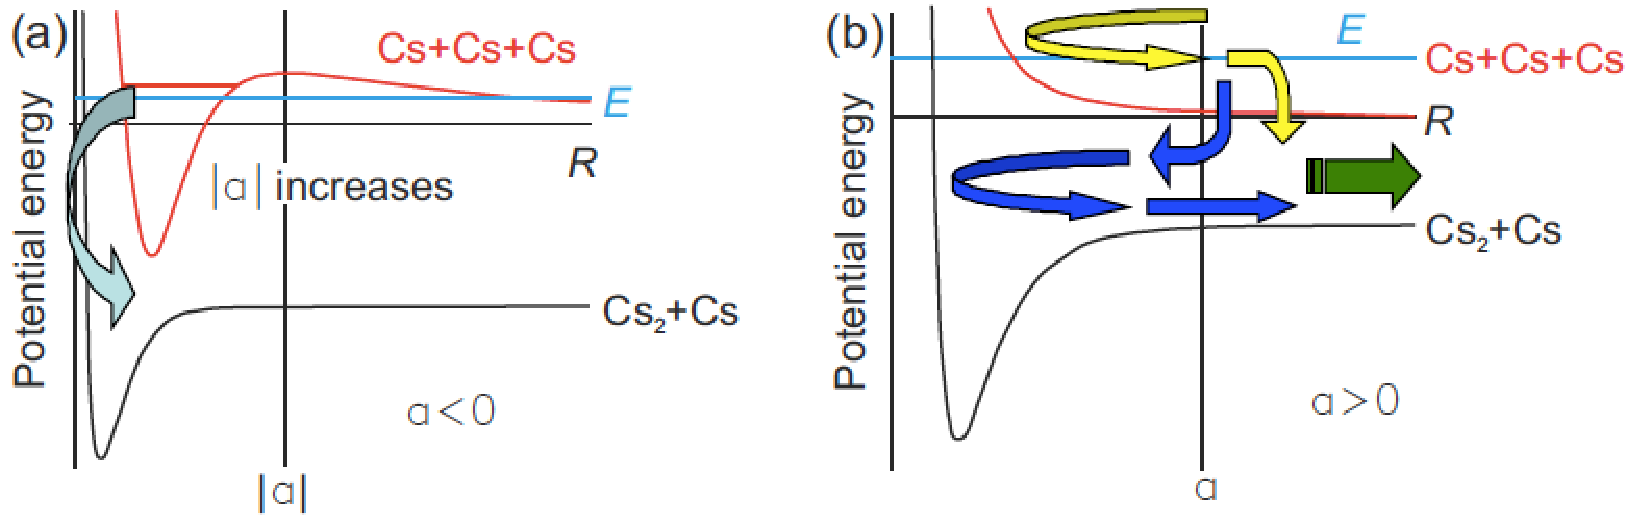
\includegraphics[width=0.75\textwidth]{Figures/efimov_recombination_coupling}
		\caption{(a) Triatomic Efimov resonance whereby the presence of an Efimov state allows for decay to a deeply bound dimer. (b) Depiction of the two channels which give rise to recombination minimum for $a>0$.  Blue path is the three incoming atoms immediately decaying at $R\approx a$, and then the atom rebounds off of the dimer.  Yellow path is all three atoms rebounding off of the hyperradial potential and then decaying to an atom and a dimer.  These paths cause interference in the outgoing path (green arrow). Adapted from \cite{Kraemer2006}}
		\label{fig:efimov_recombin_coupling}
	\end{figure}
	%\end{comment}

In the limit of large scattering lengths the three-body loss coefficient can be written as
	\begin{equation}\label{eq:3b_recombination}
		L_{3}=n_{l}\alpha_{rec}=n_{l}C(a)\frac{\hbar a^{4}}{m}
	\end{equation} 
When written in this fashion the general scaling of $L_{3}\propto a^{4}$ is separated from the non-trivial physics contain within the dimensionless $C(a)$ parameter.  This parameter has been calculated within the framework of effective field theory, and it is able to give a quantitative description of the recombination processes described above \cite{Braaten_2006}\cite{Bedaque2000}\cite{Braaten2001}\cite{Braaten2004}.  These calculations yield the following
	\begin{equation}\label{eq:C(a)}
		C(a)=\left\{\begin{array}{rl}
		4590\sinh(2\eta_{-})/[\sin^{2}[s_{0}\ln(a/a_{-})]+\sinh^{2}\eta_{-}] & \text{if } a<0\\
		67.1e^{-2\eta_{+}}(\sin^{2}[s_{0}\ln(a/a_{+})]+\sinh^{2}\eta_{+})+16.8(1-e^{-4\eta_{+}}) & \text{if } a>0
		\end{array}\right.
	\end{equation}
where the $\eta_{\pm}$ are inelasticity parameters that describe the width of the Efimov states for positive and negative scattering lengths.  The finite width arises because of the existence of decay channels to deep dimer states which give the Efimov  trimers a finite lifetime.  An order of magnitude estimate for the width of the shallowest Efimov states is given by $\eta\hbar^{2}/ma^{2}$.  More generally, the width is proportional to the binding energy, and the geometric scaling of the binding energy (see Eq. \ref{eq:Efimov_trimer_binding_E}) implies scaling of the widths as well \cite{Braaten2008}\cite{Nielsen2002}.  This inelasticity parameter is not associated with decay to a specific dimer state, instead it absorbs the cumulative effect of many possible decay channels to deeper bound dimers into a single parameter \cite{Braaten_2006}.  In addition, it is important to note that $C(a)$ exhibits the log-periodic given by $C(a)=C(e^{\pi/s_{0}}a)\approx C(22.7a)$.  This log-periodic behavior is a hallmark of Efimov physics.
	
	
		%\begin{comment}
		\begin{figure}
			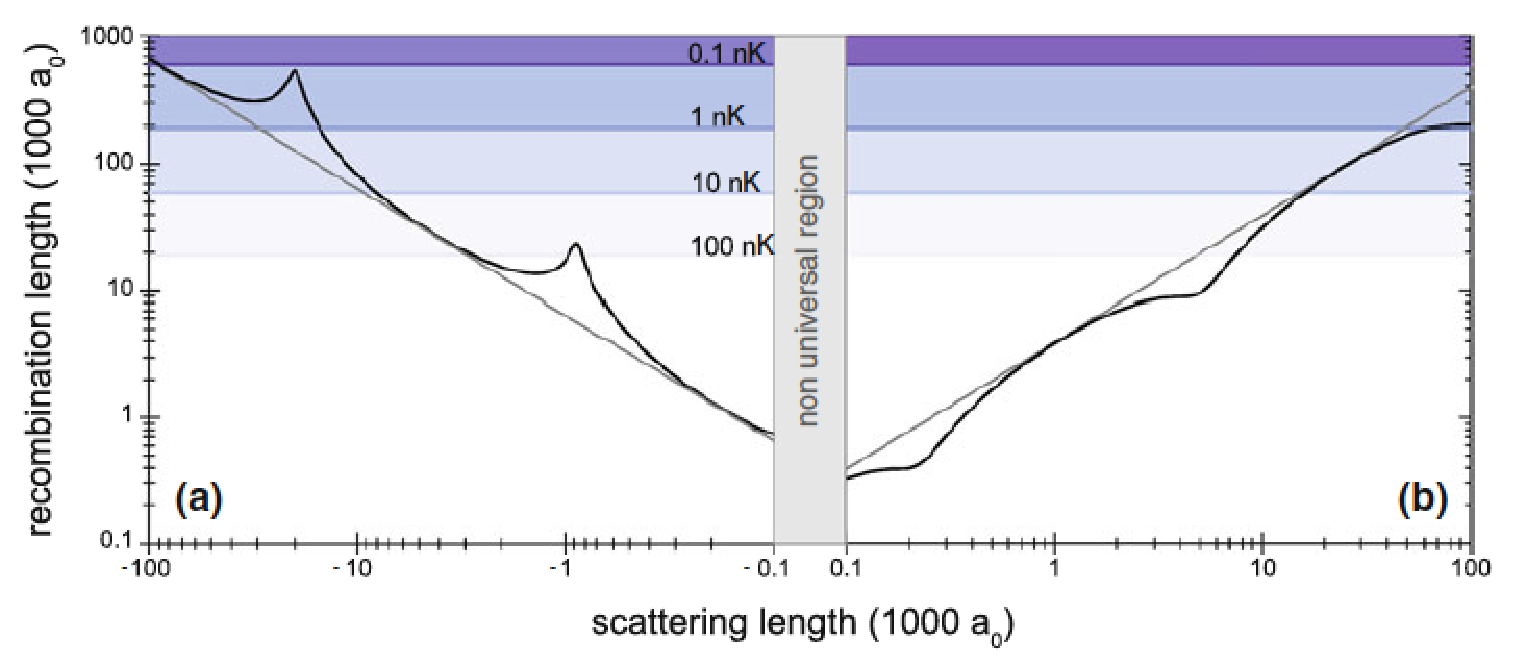
\includegraphics[width=0.8\textwidth]{Figures/recombination_length}
			\caption{Recombination length as a function of scattering length as derived from effective field theory. The parameters $a_{\pm}$ and $\eta_{\pm}$ were chosen to correspond to the Cs Efimov features of \cite{Kraemer2006_1st_observ}. The unitary recombination length is also shown as colored lines for various temperatures. Adapted from \cite{Ferlaino2011}.}
			\label{fig:recombination_length}
		\end{figure}
		%\end{comment}
A convenient way to characterize the three-body loss coefficient is through the so-called recombination length 
\cite{Ferlaino2011}, which is given by
	\begin{equation}\label{eq:recombination_length_defined}
		\rho_{3}=\sqrt[\leftroot{-2}\uproot{2}4]{\frac{2m}{\sqrt{3}\hbar}L_{3}}
	\end{equation}
The main purpose of introducing the recombination length is to reduce the $a^{4}$ scaling of $L_{3}$ to a linear relationship, $\rho_{3}=1.36\sqrt[\leftroot{-3}\uproot{3}4]{C(a)}|a|$, where $n_{l}$ has been set to a value of three \cite{Ferlaino2011}\cite{Esry1999}.  The recombination length is plotted in Fig. \ref{fig:recombination_length}.  For $a<0$, the recombination length resonantly increases whenever an Efimov trimer couples to the triatomic threshold at $a=e^{(\pi/s_{0})n}a_{-}^{(0)}$, and for $a>0$, it decreases due to destructive interference in the atom-dimer decay channel at $a=a_{+}^{(n)}$. 

Thus far, the temperature dependence of recombination has not been considered.  In the zero-temperature limit the three-body loss rate coefficient $L_{3}$ scales as $a^{4}$ as $|a|$ is increased.  However, at finite temperature, $L_{3}$ saturates when the scattering length becomes comparable to the thermal de Broglie wavelength given by $\lambda_{th}=h/\sqrt{2\pi m k_{B}T}$ \cite{Rem2013} \cite{Li2012}.  This saturation at the thermal de Broglie wavelength is equivalent to the unitary limit, and its presence implies that for a given temperature there is a maximum recombination length that can be resolved, $L_{3}\approx\hbar a^{4}/m\approx\hbar^{5}/m^{3}(k_{B}T)^{2}$ \cite{DIncao2004}.  The scaling of $L_{3}\propto 1/T^{2}$ has been observed, and is in good agreement with experimental evidence \cite{Rem2013}.  In Fig. \ref{fig:recombination_length} the temperature limited recombination length is plotted temperatures from 100 nK to 0.1 nK for Cs.  If there was no temperature limitation, then one would be able to see an infinite number of resonances as the scattering length is increased, however at temperatures of a few nK the second triatomic resonance for $a<0$ is just able to be resolved.  This represents a very significant hurdle in the observation of Efimov states \cite{D'Incao2009} in part because cooling to such temperatures is certainly non-trivial. In light of this, the time between the first observation of a confirmed Efimov resonance \cite{Kraemer2006_1st_observ} and the confirmation of the second Efimov resonance in Cs \cite{Huang2014} is understandable.



%**************************************************************************************
\section{Observation of Second Efimov State}

	\begin{figure}
		\centering
		\begin{subfigure}[b]{0.45\textwidth}
			\caption{}
			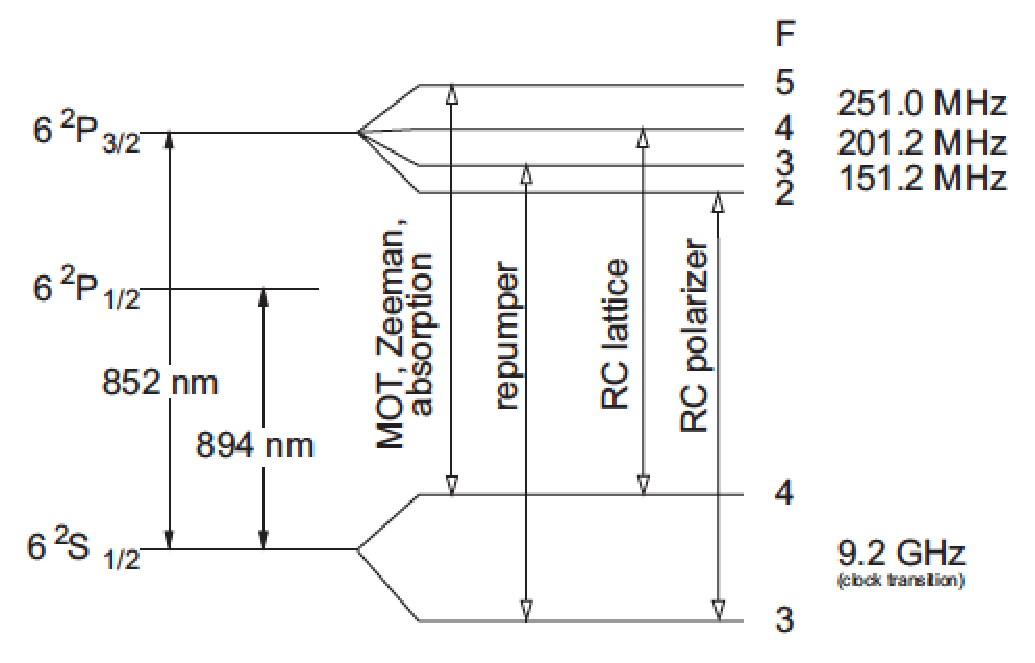
\includegraphics[width=\textwidth]{Figures/Cs_level_diagram}
			\label{fig:Cs_level_diagram}
		\end{subfigure}
		\begin{subfigure}[b]{0.29\textwidth}
			\caption{}
			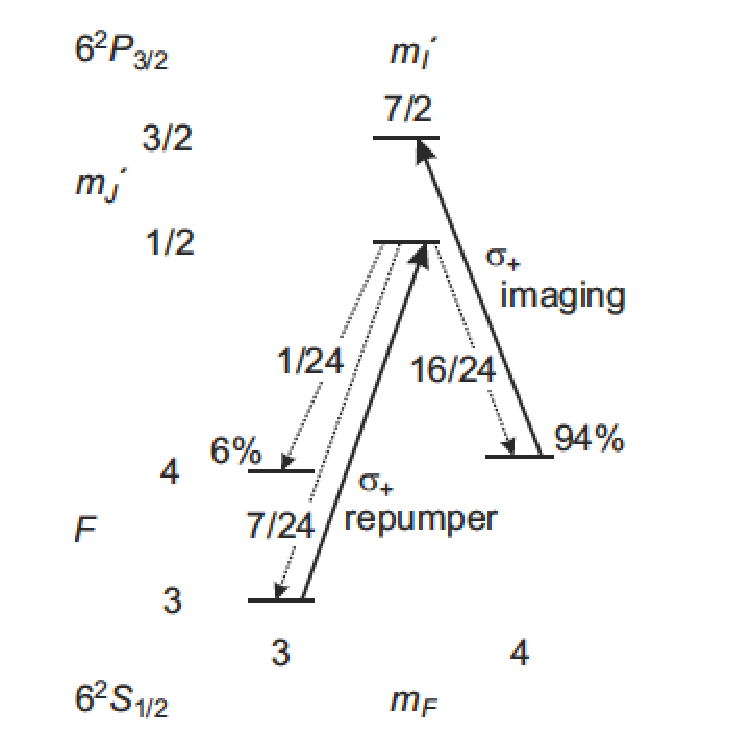
\includegraphics[width=\textwidth]{Figures/Imaging_Transitions}
			\label{fig:imaging_transitions}
		\end{subfigure}
		\caption{(a) Level diagram for $^{133}\text{Cs}$.  The transitions used in various stages of the experiment performed by the Grimm group are labeled.  Adapted from \cite{Herbig2005}. (b) Transitions used for absorption imaging.  Dotted lines represent decay channels from $\ket{m'_{J}=1/2,m'_{I}=7/2}$, and their relative probabilities are shown. Adapted from \cite{Berninger2011_thesis}.}
	\end{figure}

	 The first confirmation of an Efimov state came in 2006 from the Grimm group at the University of Innsbr\"{u}ck \cite{Kraemer2006_1st_observ}.  However, it wasn't until recently that they were able to confirm the existence of a second Efimov state, and by doing so they were able to directly test the scaling factor experimentally $e^{\pi/s_{0}}\approx22.7$ \cite{Huang2014}.  They were able to measure this Efimov state by using a gas of $^{133}\text{Cs}$ which had been cooled to a temperature of 5-7 nK.
	 
	 The procedure they use for cooling is as follows \cite{Berninger2011} \cite{Herbig2005}.  Initially, $^{133}\text{Cs}$ atoms are evaporated in an oven and are collimated through nozzle of diameter 1.5mm, forming an effusive beam of opening angle $6\,^{\circ}$.  From the oven they are sent into a Zeeman slower tube where they are slowed by a counter-propagating laser which is red-detuned by 50 MHz from the $^{2}S_{1/2}(F=4)\rightarrow$ $^{2}P_{3/2}(F'=5)$ transition, shown in Fig. \ref{fig:Cs_level_diagram}. This loads a magneto-optical trap (MOT) at a rate of $10^{7}$ atoms/s.  During loading the MOT is red-detuned by 4.5 MHz with a field gradient of 7.8 G/cm.  After compressing the MOT and an optical molasses phase where the detuning is 90MHz, the temperature has reached 10$\mu\text{K}$.  They then proceed to Raman sideband cooling by capturing the atoms in a 3D optical lattice, formed by four lasers resonant with the $^{2}S_{1/2}(F=4)\rightarrow ^{2}P_{3/2}(F'=4)$ transition.  Another beam is used to polarize the atoms into the $\ket{F=3,m_{F}=3}$ state. The polarizing beam is 7 MHz blue detuned to account for the light shift due to the lattice potential.
	 
	 The atomic cloud is then loaded into an optical dipole trap combined with magnetic levitation to cancel the influences of gravity.  The optical dipole trap is provided by $\text{CO}_{2}$ lasers at 10.6 $\mu m$ at 85 W each.  After 2 s of plain evaporation, the atoms are loaded into a tightly focused 1064 nm crossed dipole trap for forced evaporation using the dimple trick \cite{Kraemer2004}.  After 15 s of forced evaporation, the optical power of the 1064 nm crossed lasers are 3.5 mW and 300 mW, and the $\text{CO}_{2}$ lasers are switched off in the first 5 s \cite{Berninger2011}.  This stage ends with the magnetic field strength at 907 G \cite{Huang2014}. One of the trapping beams is adiabatically removed and the intensity is decreased in the other to open the trap, thus lowering the temperature. The final trap is nearly isotropic with a mean trap frequency of $\overline{\omega}/2\pi=2.6$ Hz, which corresponds to a length of approximately 5 $\mu m$.  The final sample consists of approximately $10^{4}$ Cs atoms at a temperature of 7 nK and a phase-space density of 0.2 \cite{Huang2014}.
	 
	 \begin{figure}
	 	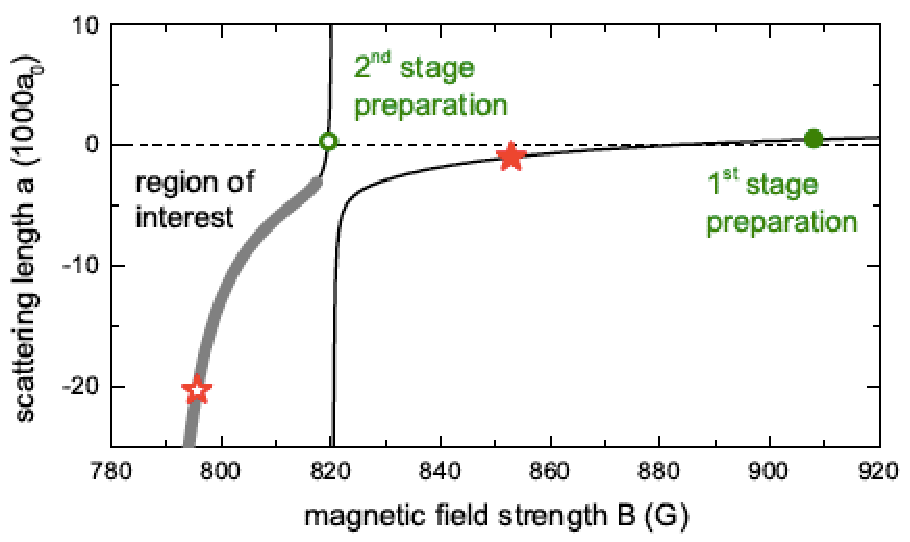
\includegraphics[width=0.7\textwidth]{Figures/experimental_steps}
	 	\caption{Region of scattering length explored for the second triatomic resonance.  The green filled circle is the field at which cooling is finished, and green circle is the field from which they explore the region of interest (thick grey line). The red filled and unfilled stars are the positions of the first and second Efimov resonance, respectively. Adapted from \cite{Huang2014}.}
	 	\label{fig:experimental steps}
	 \end{figure}
	 
	 At this point, the setup is complete and the measurement begins.  The goal is to observe the presence of a triatomic Efimov resonance that corresponds to the second Efimov state.  The scattering length at which the first Efimov resonance was seen at was $a^{(0)}_{-}=-963a_{0}$ \cite{Berninger2011}.  Thus, the scattering length where the resonance associated with the second Efimov state should occur would be located at $a=22.7a^{(0)}_{-}=-21900a_{0}$.  Following the model for the scattering length versus magnetic field \cite{Berninger2013}, they select a region of interest shown in Figs. \ref{fig:a_vs_B_M2012} and \ref{fig:experimental steps}, which corresponds to a magnetic field between 818 G and 757 G.
	 
	 	\begin{comment}
	 	\begin{figure}
	 		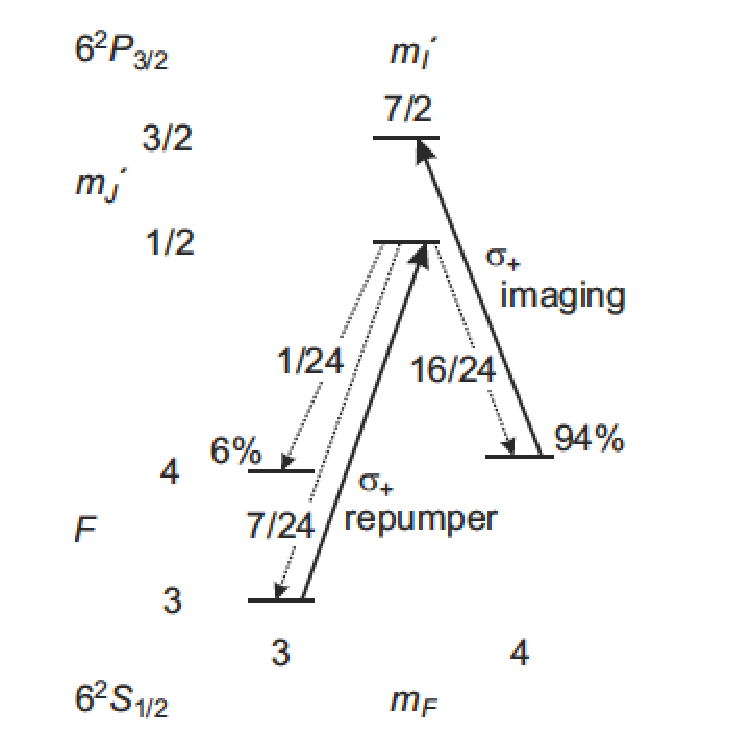
\includegraphics[width=0.4\textwidth]{Figures/Imaging_Transitions}
	 		\caption{Transitions used for absorption imaging.  Dotted lines represent decay channels from $\ket{m'_{J}=1/2,m'_{I}=7/2}$, and their relative probabilities are shown. Adapted from \cite{Berninger2011_thesis}.}
	 	\end{figure}
	 	\end{comment}
	 	
	 Beginning from the final preparation field, they ramp to the target magnetic field within 10 ms and wait for anywhere between tens of milliseconds to several seconds.  The maximum hold time corresponds to half of the atoms being lost.  To observe the number of atoms lost after the variable hold time, they perform absorption imaging \cite{Huang2014}.  Whereby resonant light illuminates the atomic cloud, and atoms scatter photons of the illuminating light generating a shadow image.  This allows for the density distribution to be mapped out.  The closed optical transition used is shown in Fig. \ref{fig:imaging_transitions}. The field at which the imaging takes place is 881.9 G \cite{Huang2014}, where there is a zero-crossing of the scattering length, see Fig. \ref{fig:experimental steps}.  At this field, the ground state $^{2}S_{1/2}$ is still described by the quantum numbers $F$ and $m_{F}$, but the good quantum numbers for the excited state $^{2}P_{3/2}$ are $m_{J}$ and $m_{I}$ (see Fig. \ref{fig:Zeeman_splitting}).  The atoms are in the state $\ket{F=3,m_{F}=3}$ initially and are then  transferred to the state $\ket{F=4,m_{F}=4}$ by the repumper light  which is resonant on the $\ket{F=3,m_{F}=3}\rightarrow\ket{m'_{J}=1/2,m'_{I}=7/2}$ transition \cite{Berninger2011_thesis}.  The majority are transferred to the $\ket{F=4,m_{F}=4}$ state, but a small number are lost to the $\ket{F=4,m_{F}=3}$ state, which is a dark state.  From the absorption imaging, they are able to extract the density profile and temperature.
	 
	 \begin{figure}
	 	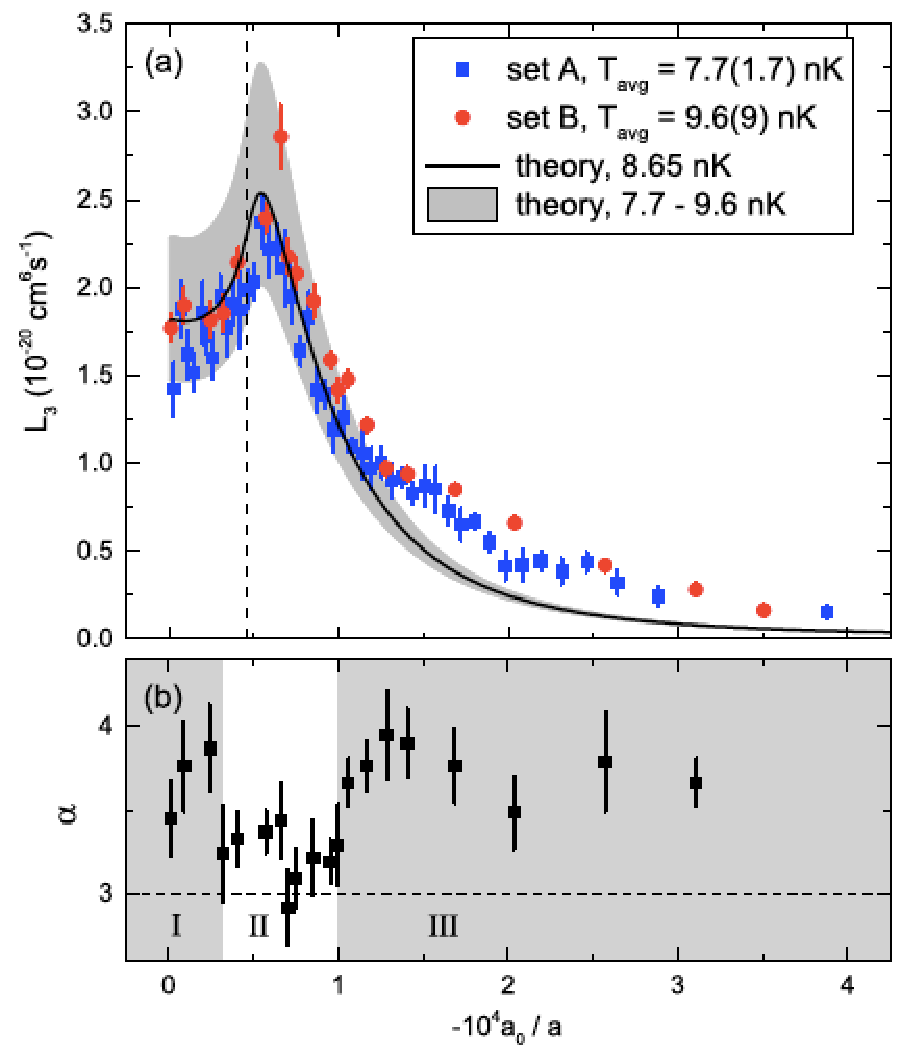
\includegraphics[width=0.6\textwidth]{Figures/second_efimov_evidence}
	 	\caption{Observation of the second Efimov resonance. (a) Three-body loss coefficient $L_{3}$ plotted as a function of $1/a$. Two sets of data are shown, and the theoretical fit is shown. The vertical dashed line is where the Efimov resonance was predicted to occur based on the scaling from the precious experiment \cite{Kraemer2006_1st_observ}. Adapted from \cite{Huang2014}}
	 	\label{fig:second_efimov_evidence}
	 \end{figure}
	 
	 By monitoring total number of atoms in the trap as a function of the delay, they are able to directly measure the recombination rate coefficient $L_{3}$ given in Eq. \ref{eq:3_body_recomination_equation}.  To extract $L_{3}$, they assume a general differential equation for $\alpha$-body losses,
	 	\begin{equation}\label{eq:alpha_body_DiffEq}
	 		\frac{\dot{N}}{N}=-L_{\alpha}\alpha^{-3/2}\bigg(\frac{N}{V}\bigg)^{\alpha-1},
	 	\end{equation}
	where the volume $V=(2\pi k_{B}T/m\overline{\omega}^{2})^{3/2}$.  By numerically integrating Eq. \ref{eq:alpha_body_DiffEq} over time, they are then able to fit the atomic number evolution with the initial number of atoms $N_{0}$, $\alpha$, and $L_{3}$ as fit parameters.  This is done for a fixed value of the scattering.  By again tuning the magnetic field through the region around where the second Efimov resonance was predicted to be, they are able to map out the behavior of $L_{3}(a)$.  The data they took is shown in Fig. \ref{fig:second_efimov_evidence}.  This data is then fit to the theoretical prediction of Eq. \ref{eq:C(a)} with corrections for finite temperature \cite{Rem2013}.  The fit agrees with the experimental data in the region of the peak, and it is thus attributed to the presence of an Efimov state coupling to the scattering threshold.  This can be further substantiated by the fact that in the region around the peak the fitted value for $\alpha$ is close to three.  This is strongly indicative that three-body losses are dominate in the region where the Efimov state is predicted to be.  
	
	From the fit to the data, they are then able to extract the peak position of the resonance.  They got a value of $a^{(1)}_{-}=-20190(1200)a_{0}$ for the second Efimov resonance and from previous work they obtained a value of $a^{(0)}_{-}=-963(11)a_{0}$.  Thus, the scaling between values is $a^{(1)}_{-}/a^{(0)}_{-}=21.0(1.3)$ which is consistent with the predicted value of 22.7.
	
	
	
	

%**************************************************************************************
\begin{comment}
\section{Experiment}
     Three body scattering experiments were first performed by Sir Rickenbacker Hageman the cat, the first of his name. Sir Ricky decided to cool the atoms so that the laserpointer would not run away as quickly as it was doing so. By cooling the atoms and applying the magnetic field he saw that the scattered in triplicate by imaging the particles with his super bionic tail. Sir Ricky has saved the day! and no other cat has been knighted since or ever will be again.
\end{comment}
\section{Conclusion}

The fairytale has certainly become a reality.  While Efimov states had been observed through resonances before, it is the confirmation of the predicted scaling behavior which is the keystone measurement in confirming Efimov's original scenario.  However, there is still much to discovered about Efimov states, and possible extensions to be made to Efimov's original scenario.  It is supposed to be a universal theory, so observation in other systems will be important. They were originally predicted in the context of nuclear physics and there are some predictions that it may be possible to observe them even in condensed matter systems \cite{Nishida2013}.  There is still a substantial amount of physics left to be discovered, and it will be exciting to watch the progress of the field.

\bibliography{candidacy_bib}

\end{document}
%**************************************************************************************